\chapter{タイミング較正によるトリガー性能の改善}
\thispagestyle{empty}
\label{chap:6}
本章では~TGC~のタイミング調整に伴った検出器性能について評価した結果を記す。特に検出器に飛来したミューオン等の荷電粒子に対し、どの程度の割合でトリガーを発行しているかを示すトリガー効率に着目し考察をする。
また、TGC~検出器でのタイミングは基本的に光速のミューオンに対し最適化されているため、速度の遅い粒子に対する感度に関しては評価手法が確立されていない。本研究では速度に依存したトリガー効率について詳細に調査することで、バンチ判定をもとにトリガー効率を推定する新たな評価手法を確立した。
以下では、タイミング調整によるトリガーの性能評価および新物理探索における評価手法についての検証結果を記す。
\section{タイミング較正に伴うミューオンのトリガー性能評価}
\chapref{chap:5}では、Run~2~データのタイミングをより詳細に見積もるためにモンテカルロシミュレーションの改良を行った。
本節では、光速のミューオンに対するタイミング較正に伴う初段シングルミューオントリガーの性能について比較した結果を示す。
\subsection{タイミング調整とトリガー効率}
初段シングルミューオントリガーにおけるトリガー効率の評価を行う。Run~2~実験データおよび$Z~→~\mu\mu$~モンテカルロサンプルを用いて、同様のイベント選別を行いトリガー効率の比較する。解析には、バイアスがかからないようにするために~$Z~→~\mu\mu$~tag~and~probe~法を用いた。トリガー効率は\equref{eq:eff}を用いて算出した。$N_{\rm{probe~muon}}$,~$N_{\rm{probe~muon}}^{\rm{triggered}}$~はそれぞれプローブミューオンの事象数、トリガー条件を満たしたプローブミューオンの事象数を表している。

\begin{align}
    \epsilon=\frac{N_{\rm{probe~muon}}^{\rm{triggered}}}{N_{\rm{probe~muon}}}
    \label{eq:eff}
\end{align}

\figref{fig:singletri}は、シングルミューオントリガーにおけるトリガー効率を比較した図である。タイミング較正前後のトリガー効率を比較すると大きな差は見られていないことがわかる。またシミュレーションと実験データとの比較でも大きな差はなく、実験データのトリガー効率を再現できていることがわかる。結果としてタイミング較正によるシングルミューオントリガーへの影響は
見られないことが確認できた。

また、\figref{fig:singletriep}は、$\eta,~\phi$~方向に区分したミューオンに対するシングルミューオントリガーのトリガー効率を示している。シミュレーションにおいては大きな変化は見られないが、実験データに関してはシミュレーションに比べると効率の低下が大きい部分が一部に観察できる。これは、デッドチェンバーにおける非効率が由来していると考えられる。
\begin{figure}[H]
        \centering   
        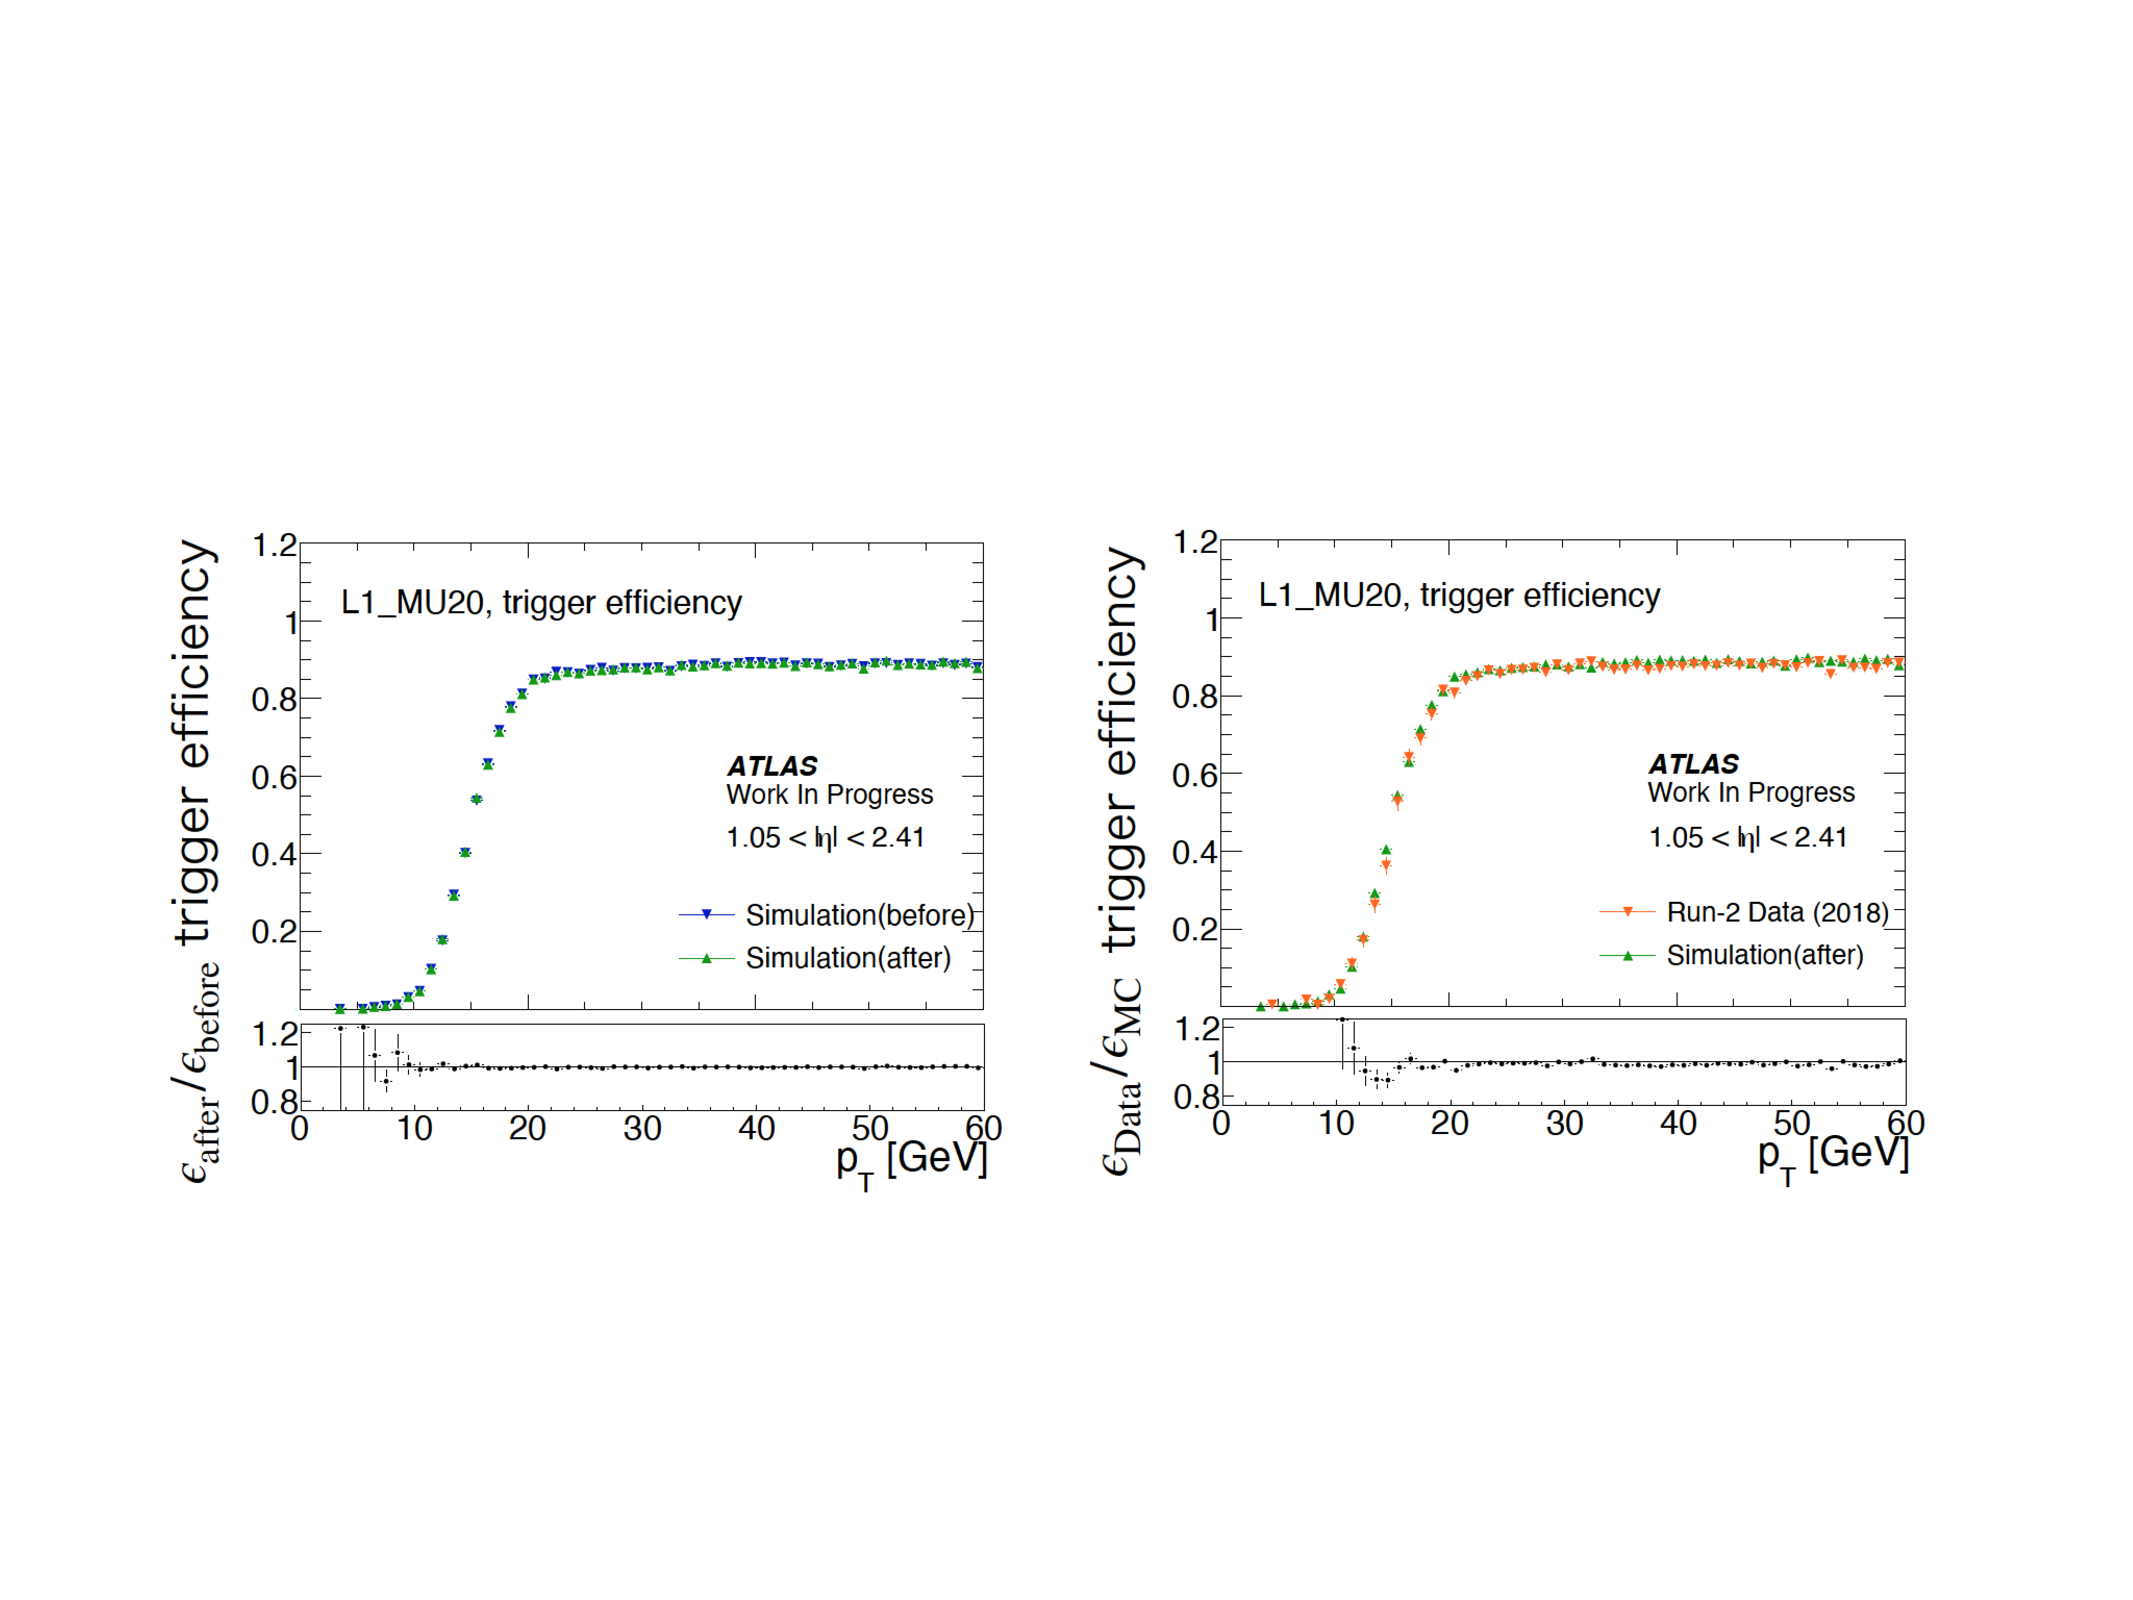
\includegraphics[width=\textwidth,page=1]{img/rec/trig.pdf}
        \caption[シングルミューオントリガーにおけるミューオンのトリガー効率の比較]{シングルミューオントリガーにおけるミューオンのトリガー効率の比較。横運動量閾値は~20~GeV。左図の青は較正前のシミュレーション、緑は較正後のシミュレーションを表す。右図の緑は較正後のシミュレーション、橙はRun~2~のデータを示す。}\label{fig:singletri}
\end{figure}

\begin{figure}[H]
        \centering   
        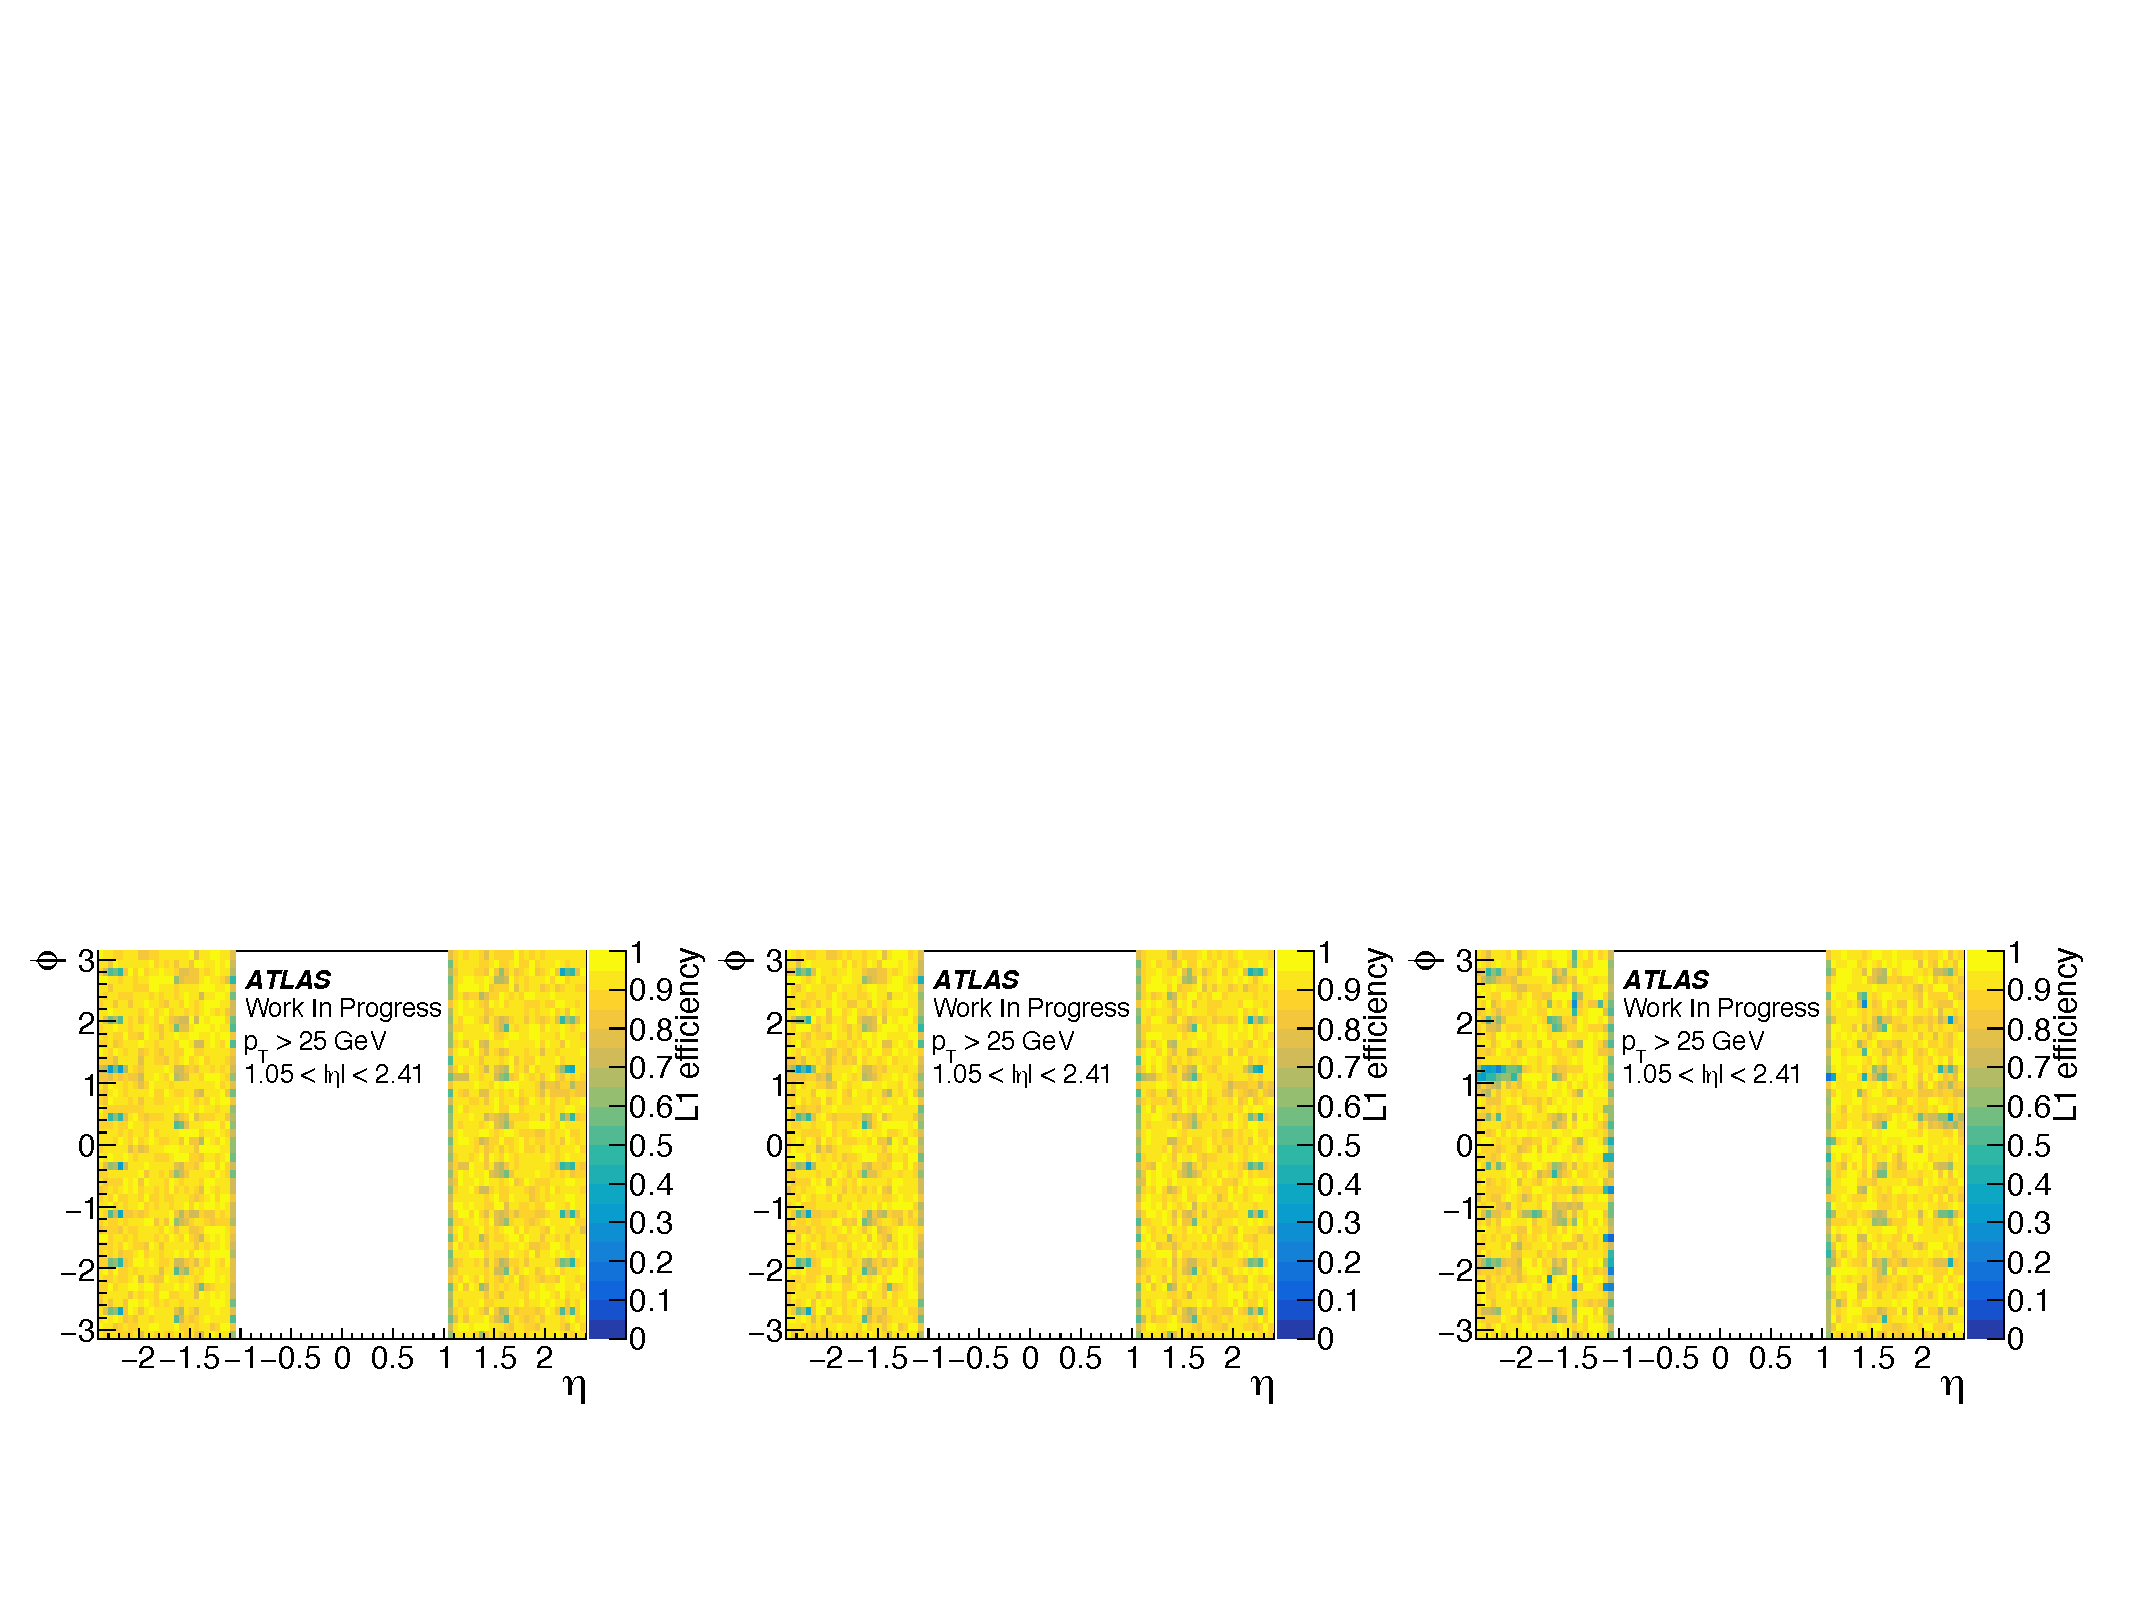
\includegraphics[width=\textwidth,page=1]{img/rec/tri1.pdf}
        \caption[$\eta, \phi$方向から見たシングルミューオントリガーにおけるトリガー効率の比較]{$\eta,~\phi$方向から見たシングルミューオントリガーにおけるトリガー効率の比較。左図は較正前のシミュレーション。中図は較正後のシミュレーション。右図は、Run~2~実験データ。}\label{fig:singletriep}
\end{figure}

\subsecref{subsec:cali}では各ステーションにおけるミューオンヒットに対するバンチ判定の割合について示した。タイミング較正前後においては前かつ基準、基準かつ次のバンチの割合が変化している。初段シングルミューオントリガーは、基準バンチでのヒットが条件となっているが、前かつ基準、基準かつ次と判定される場合でもトリガー条件を満たせばトリガー判定が行われる。従って実験データ、シミュレーションともに前かつ基準、基準かつ次を含んだ基準バンチの割合に大きな差がないため、シングルミューオントリガーには大きな影響はなかったと考えられる。
\section{タイミング較正に伴うスタウ粒子サンプルのトリガー性能評価}
Run~2~後半に新たに導入された重い荷電粒子探索用トリガーは、次のバンチと識別された速度の遅い粒子に対して感度を持つ。したがってバンチ識別のタイミングが~TGC~検出器の遅延パラメータの影響で変化した場合、トリガー可能な~$\beta$~の領域が変化する可能性が考えられる。本節では、スタウ粒子のシミュレーションサンプルを用い、重い荷電粒子探索用トリガーにおけるタイミング調整に伴ったトリガー性能についての比較を行った。
\subsection{タイミング較正に伴ったトリガー効率の比較}\label{sec:tribeta}
タイミング較正前後のシミュレーションにおける粒子速度に依存したトリガー効率を\figref{fig:tribeta}に示した。較正前後においてバンチ判定の分布の変化に伴い、トリガーできる~$\beta$~の領域が変化していることがわかる。これは、タイミング較正によりバンチを判定するタイミングに違いがあることが影響していると示唆される。また、$\beta=1.0$~の光速の領域においては較正前後においてトリガー効率に変化はないことがわかる。

また、\figref{fig:tript}、\figref{fig:trieta}はそれぞれ運動量、$\eta$~に依存したスタウサンプルに対するトリガー効率を示している。タイミング較正前後における各トリガー効率を比較するとトリガーできている領域に違いがみられる。トリガー領域に違いがみられる原因としては~$\beta$~方向のトリガー領域の変化によるものであると考えられる。詳細は\figref{fig:tripteta}、\figref{fig:triptbeta}、\figref{fig:trietabeta}を用いて考察する。
\figref{fig:tripteta}は~$p_{\rm{T}},~\eta$~方向に区分したトリガー事象の分布、\figref{fig:triptbeta}は~$p_{\rm{T}},~\beta$~方向に区分したトリガー事象の分布、\figref{fig:trietabeta}は~$\eta,~\beta$~方向に区分したトリガー事象の分布を示している。グラフからそれぞれの変数に対して依存性がみられ、事象数としてはシミュレーション間において同一のふるまいを示しているが、タイミング較正によりトリガー事象の分布に変化がみられることがわかる。\figref{fig:tript}におけるふるまいの変化は、\figref{fig:triptbeta}より、トリガー可能な~$\beta$~の領域の変化と$p_{\rm{T}}$~と~$\beta$~の依存性による影響であることがわかる。 
\begin{figure}[H]
    \begin{minipage}{0.49\hsize}
    \centering   
    \includegraphics[width=\textwidth,page=2]{img/rec/stau_600_ori.pdf}
    \subcaption{}
    \end{minipage}
    \begin{minipage}{0.49\hsize}
    \centering   
    \includegraphics[width=\textwidth,page=2]{img/rec/stau_600.pdf}
    \subcaption{}
    \end{minipage}
    \caption[スタウ粒子サンプルにおけるタイミング較正前後の速度に依存したトリガー効率の比較]{スタウ粒子サンプルにおけるタイミング較正前後の速度に依存したトリガー効率の比較。赤は横運動量閾値~10~GeV~の~L1~シングルミューオントリガー、青は横運動量閾値~10~GeV~の遅い荷電粒子探索用トリガーのトリガー効率を示す。(a)~較正前のシミュレーション。(b)~較正後のシミュレーション。}\label{fig:tribeta}
\end{figure}
\begin{figure}[H]
    \begin{minipage}{0.49\hsize}
    \centering   
    \includegraphics[width=\textwidth,page=4]{img/rec/stau_600_ori.pdf}
    \subcaption{}
    \end{minipage}
    \begin{minipage}{0.49\hsize}
    \centering   
    \includegraphics[width=\textwidth,page=4]{img/rec/stau_600.pdf}
    \subcaption{}
    \end{minipage}
    \caption[スタウ粒子サンプルにおけるタイミング較正前後の横運動量に依存したトリガー効率の比較]{スタウ粒子サンプルにおけるタイミング較正前後の横運動量に依存したトリガー効率の比較。黒(●)は~L1~ミューオントリガー、赤(●)は横運動量閾値~10~GeV~の~L1~シングルミューオントリガー、青(●)は横運動量閾値~10~GeV~の遅い荷電粒子探索用トリガー、青(▲)は~MET~トリガーを要求しない遅い荷電粒子探索用トリガーのトリガー効率を示す。(a)~較正前のシミュレーション。(b)~較正後のシミュレーション。}\label{fig:tript}
\end{figure}
\begin{figure}[H]
    \begin{minipage}{0.49\hsize}
    \centering   
    \includegraphics[width=\textwidth,page=9]{img/rec/stau_600_ori.pdf}
    \subcaption{}
    \end{minipage}
    \begin{minipage}{0.49\hsize}
    \centering   
    \includegraphics[width=\textwidth,page=9]{img/rec/stau_600.pdf}
    \subcaption{}
    \end{minipage}
    \caption[スタウ粒子サンプルにおけるタイミング較正前後の~$\eta$~に依存したトリガー効率の比較]{スタウ粒子サンプルにおけるタイミング較正前後の~$\eta$~に依存したトリガー効率の比較。黒(●)は~L1~ミューオントリガー、赤(●)は横運動量閾値~10~GeV~の~L1~シングルミューオントリガー、青(●)は横運動量閾値~10~GeV~の遅い荷電粒子探索用トリガー、青(▲)は~MET~トリガーを要求しない遅い荷電粒子探索用トリガーのトリガー効率を示す。(a)~較正前のシミュレーション。(b)~較正後のシミュレーション。}\label{fig:trieta}
\end{figure}

\begin{figure}[H]
    \begin{minipage}{0.49\hsize}
    \centering   
    \includegraphics[width=\textwidth,page=14]{img/rec/stau_600_ori.pdf}
    \subcaption{}
    \end{minipage}
    \begin{minipage}{0.49\hsize}
    \centering   
    \includegraphics[width=\textwidth,page=14]{img/rec/stau_600.pdf}
    \subcaption{}
    \end{minipage}
    \caption[スタウ粒子サンプルにおけるタイミング較正前後の~$\eta$~および横運動量に依存したトリガー効率の比較]{スタウ粒子サンプルにおけるタイミング較正前後の~$\eta$~および横運動量に依存したトリガー効率の比較。黒の四角は事象数、赤は横運動量閾値~10~GeV~の~L1~シングルミューオントリガー、青は横運動量閾値~10~GeV~の遅い荷電粒子探索用トリガーを通過した事象を示す。(a)~較正前のシミュレーション。(b)~較正後のシミュレーション。}\label{fig:tripteta}
\end{figure}
\begin{figure}[H]
    \begin{minipage}{0.49\hsize}
    \centering   
    \includegraphics[width=\textwidth,page=15]{img/rec/stau_600_ori.pdf}
    \subcaption{}
    \end{minipage}
    \begin{minipage}{0.49\hsize}
    \centering   
    \includegraphics[width=\textwidth,page=15]{img/rec/stau_600.pdf}
    \subcaption{}
    \end{minipage}
    \caption[スタウ粒子サンプルにおけるタイミング較正前後の速度および横運動量に依存したトリガー効率の比較]{スタウ粒子サンプルにおけるタイミング較正前後の速度および横運動量に依存したトリガー効率の比較。黒の四角は事象数、赤は横運動量閾値~10~GeV~の~L1~シングルミューオントリガー、青は横運動量閾値~10~GeV~の遅い荷電粒子探索用トリガーを通過した事象を示す。(a)~較正前のシミュレーション。(b)~較正後のシミュレーション。}\label{fig:triptbeta}
\end{figure}
\begin{figure}[H]
    \begin{minipage}{0.49\hsize}
    \centering   
    \includegraphics[width=\textwidth,page=16]{img/rec/stau_600_ori.pdf}
    \subcaption{}
    \end{minipage}
    \begin{minipage}{0.49\hsize}
    \centering   
    \includegraphics[width=\textwidth,page=16]{img/rec/stau_600.pdf}
    \subcaption{}
    \end{minipage}
    \caption[スタウ粒子サンプルにおけるタイミング較正前後の速度および~$\eta$~に依存したトリガー効率の比較]{スタウ粒子サンプルにおけるタイミング較正前後の速度および~$\eta$~に依存したトリガー効率の比較。黒の四角は事象数、赤は横運動量閾値~10~GeV~の~L1~シングルミューオントリガー、青は横運動量閾値~10~GeV~の遅い荷電粒子探索用トリガーを通過した事象を示す。(a)~較正前のシミュレーション。(b)~較正後のシミュレーション。}\label{fig:trietabeta}
\end{figure}

\subsection{粒子質量の違いによるトリガー効率の比較}\label{sec:trimass}
本研究においては、スタウ粒子のシミュレーションサンプルとして、質量が~600~GeV~および~1000~GeV~のサンプルを使用した。タイミング較正後のシミュレーションを利用し、質量の違いによるトリガー効率への影響について考察する。
\figref{fig:tribeta6}は、速度に依存したトリガー効率の変化を比較したものである。スタウ粒子サンプルの質量が異なることで、トリガーできる~$\beta$~の領域に変化は見られない。各変数における分布のの詳細については\secref{sec:tribeta}での比較の仕方と同様に行う。
\begin{figure}[H]
    \begin{minipage}{0.49\hsize}
    \centering   
    \includegraphics[width=\textwidth,page=2]{img/rec/stau_600.pdf}
    \subcaption{}
    \end{minipage}
    \begin{minipage}{0.49\hsize}
    \centering   
    \includegraphics[width=\textwidth,page=2]{img/rec/stau_1000.pdf}
    \subcaption{}
    \end{minipage}
    \caption[質量の異なるスタウ粒子サンプルにおける速度に依存したトリガー効率の比較]{質量の異なるスタウ粒子サンプルにおける速度に依存したトリガー効率の比較。タイミング較正後のシミュレーションを利用している。赤は横運動量閾値~10~GeV~の~L1~シングルミューオントリガー、青は横運動量閾値~10~GeV~の遅い荷電粒子探索用トリガーのトリガー効率を示す。(a)~質量~600~GeV。(b)~質量~1000~GeV。}\label{fig:tribeta6}
\end{figure}
\figref{fig:tript6}を見ると、まず~L1~トリガー全体として取得できる~$p_{\rm{T}}$~の領域が異なっていることがわかる。これは同じ粒子速度である場合でも、質量が大きくなると~$p_{\rm{T}}$~の値が大きくなることに由来する。同じ~$p_{\rm{T}}$~の場合、質量が大きい方が粒子速度が遅くなるため、バンチ判定においては次のバンチの割合が大きくなる。
また、\figref{fig:tribeta6}に~$p_{\rm{T}}$,~$\beta$~の~トリガー領域と事象数の分布を示した。\secref{sec:tribeta}のときとは異なり、事象が観測される領域についても変化していることがわかる。
以上の理由により質量が大きいサンプルの方がトリガーできる~$p_{\rm{T}}$~の領域が~$p_{\rm{T}}$~の高い方向にシフトしている。

\figref{fig:trieta6}に関しても、質量差による影響が確認でき~$\eta$~方向においてもトリガー領域に違いがみられる。
\figref{fig:tripteta6}、\figref{fig:trietabeta6}に~$p_{\rm{T}}$,~$\eta$~および~$p_{\rm{T}}$,~$\beta$~の~トリガー領域と事象数の分布を示した。
\begin{figure}[H]
    \begin{minipage}{0.49\hsize}
    \centering   
    \includegraphics[width=\textwidth,page=4]{img/rec/stau_600.pdf}
    \subcaption{}
    \end{minipage}
    \begin{minipage}{0.49\hsize}
    \centering   
    \includegraphics[width=\textwidth,page=4]{img/rec/stau_1000.pdf}
    \subcaption{}
    \end{minipage}
    \caption[質量の異なるスタウ粒子サンプルにおける横運動量に依存したトリガー効率の比較]{質量の異なるスタウ粒子サンプルにおける横運動量に依存したトリガー効率の比較。タイミング較正後のシミュレーションを利用している。黒(●)は~L1~ミューオントリガー、赤(●)は横運動量閾値~10~GeV~の~L1~シングルミューオントリガー、青(●)は横運動量閾値~10~GeV~の遅い荷電粒子探索用トリガー、青(▲)は~MET~トリガーを要求しない遅い荷電粒子探索用トリガーのトリガー効率を示す。(a)~質量~600~GeV。(b)~質量~1000~GeV。}\label{fig:tript6}
\end{figure}
\begin{figure}[H]
    \begin{minipage}{0.49\hsize}
    \centering   
    \includegraphics[width=\textwidth,page=9]{img/rec/stau_600.pdf}
    \subcaption{}
    \end{minipage}
    \begin{minipage}{0.49\hsize}
    \centering   
    \includegraphics[width=\textwidth,page=9]{img/rec/stau_1000.pdf}
    \subcaption{}
    \end{minipage}
    \caption[質量の異なるスタウ粒子サンプルにおける~$\eta$~に依存したトリガー効率の比較]{質量の異なるスタウ粒子サンプルにおける~$\eta$~に依存したトリガー効率の比較。タイミング較正後のシミュレーションを利用している。黒(●)は~L1~ミューオントリガー、赤(●)は横運動量閾値~10~GeV~の~L1~シングルミューオントリガー、青(●)は横運動量閾値~10~GeV~の遅い荷電粒子探索用トリガー、青(▲)は~MET~トリガーを要求しない遅い荷電粒子探索用トリガーのトリガー効率を示す。(a)~質量~600~GeV。(b)~質量~1000~GeV。}\label{fig:trieta6}
\end{figure}
\begin{figure}[H]
    \begin{minipage}{0.49\hsize}
    \centering   
    \includegraphics[width=\textwidth,page=14]{img/rec/stau_600.pdf}
    \subcaption{}
    \end{minipage}
    \begin{minipage}{0.49\hsize}
    \centering   
    \includegraphics[width=\textwidth,page=14]{img/rec/stau_1000.pdf}
    \subcaption{}
    \end{minipage}
    \caption[質量の異なるスタウ粒子サンプルにおける~$\eta$~および横運動量に依存したトリガー効率の比較]{質量の異なるスタウ粒子サンプルにおける~$\eta$~および横運動量に依存したトリガー効率の比較。タイミング較正後のシミュレーションを利用している。黒の四角は事象数、赤は横運動量閾値~10~GeV~の~L1~シングルミューオントリガー、青は横運動量閾値~10~GeV~の遅い荷電粒子探索用トリガーを通過した事象を示す。(a)~質量~600~GeV。(b)~質量~1000~GeV。}\label{fig:tripteta6}
\end{figure}
\begin{figure}[H]
    \begin{minipage}{0.49\hsize}
    \centering   
    \includegraphics[width=\textwidth,page=15]{img/rec/stau_600.pdf}
    \subcaption{}
    \end{minipage}
    \begin{minipage}{0.49\hsize}
    \centering   
    \includegraphics[width=\textwidth,page=15]{img/rec/stau_1000.pdf}
    \subcaption{}
    \end{minipage}
    \caption[質量の異なるスタウ粒子サンプルにおける速度および横運動量に依存したトリガー効率の比較]{質量の異なるスタウ粒子サンプルにおける速度および横運動量に依存したトリガー効率の比較。タイミング較正後のシミュレーションを利用している。黒の四角は事象数、赤は横運動量閾値~10~GeV~の~L1~シングルミューオントリガー、青は横運動量閾値~10~GeV~の遅い荷電粒子探索用トリガーを通過した事象を示す。(a)~質量~600~GeV。(b)~質量~1000~GeV。}\label{fig:triptbeta6}
\end{figure}
\begin{figure}[H]
    \begin{minipage}{0.49\hsize}
    \centering   
    \includegraphics[width=\textwidth,page=16]{img/rec/stau_600.pdf}
    \subcaption{}
    \end{minipage}
    \begin{minipage}{0.49\hsize}
    \centering   
    \includegraphics[width=\textwidth,page=16]{img/rec/stau_1000.pdf}
    \subcaption{}
    \end{minipage}
    \caption[質量の異なるスタウ粒子サンプルにおける速度および~$\eta$~に依存したトリガー効率の比較]{質量の異なるスタウ粒子サンプルにおける速度および~$\eta$~に依存したトリガー効率の比較。タイミング較正後のシミュレーションを利用している。黒の四角は事象数、赤は横運動量閾値~10~GeV~の~L1~シングルミューオントリガー、青は横運動量閾値~10~GeV~の遅い荷電粒子探索用トリガーを通過した事象を示す。(a)~質量~600~GeV。(b)~質量~1000~GeV。}\label{fig:trietabeta6}
\end{figure}
\subsection{速度に依存したトリガー効率の新しい見積もり手法の構築}\label{sec:est}
\secref{sec:tribeta}、\secref{sec:trimass}では、シミュレーションを用いて、タイミング較正に伴うトリガー効率への影響およびサンプルの質量の違いに伴うトリガー効率への影響について考察してきた。タイミング較正前後の比較においては、バンチ判定を行うタイミングの変化に伴いトリガー可能な~$\beta$~の領域に違いがみられることを示した。

シミュレーションを用いて得られた粒子速度に依存したトリガー効率を評価するためには、実験データにおけるトリガー効率との比較が必要となる。しかし実験データにおいて~TGC~検出器で観測される事象は、ほとんどが光速のミューオンであり、速度の遅い荷電粒子は未観測である。すなわち実験データを直接解析しても、速度の遅い領域のトリガー効率を得ることはできない。
そのため、トリガー効率を見積もるには新たな発想で別の方法を構築する必要がある。
本節では、実験データにおける速度に依存したトリガー効率を見積もるために構築した新たな評価手法について
説明する。
\subsubsection{確率分布関数の定義方法}\label{sec:pro}
TGC~検出器では、粒子の信号ごとにバンチ識別を行っている。
光速のミューオンを仮定した場合、ほとんどが基準バンチで判定されるが\chapref{chap:4}でも述べた通り、信号が検出されるタイミングには一定の揺らぎがある。統計的に十分なミューオン事象を~TGC~で検出したとする。以上の場合それぞれのミューオンごとにタイミングの揺らぎがあり検出されるタイミングは異なるが、ヒットのタイミングを時間の関数としてみれば、ある確率分布に従って観測されるということが仮定できる。
この確率分布は、バンチ判定をもとに近似的に決定することができる。\figref{fig:rectune}はタイミング較正を行ったシミュレーションにおけるバンチ判定の分布をもとに定義した確率分布関数である。BCID~ゲートとヒットタイミングの関係から算出することが可能である。\subsecref{subsec:cali}では、シミュレーションにおける~M1~ステーションのバンチ判定分布割合について示した。確率分布関数は、この割合に従って定義される。バンチを判定する~BCID~ゲートを設定どおり定義し、得られているバンチ判定分布を満たすように確率分布関数の形を決定する。本研究では確率分布関数を近似的に三角形として定義している。以下で三角形の詳細な定義方法についてまとめる。
\begin{itemize}
\item 前かつ基準バンチ、基準バンチ、基準かつ次のバンチの割合を示す $\it{R}_{\rm{P.\& C.}}$, $\it{R}_{\rm{C.}}$, $\it{R}_{\rm{C.\& N.}}$ がバンチ判定の分布割合を満たすような三角形を考える。確率分布は~M1~におけるバンチ判定の分布を基準として算出する。
\item 三角形の頂点を決定する(\figref{fig:rectune}の三角形における上部の頂点)。頂点は任意の座標で決めることができるが、今回は基準バンチの中心を頂点とした。
\item 決定した頂点を固定した上で、バンチ判定の分布割合を満たすように残りの 2 頂点を決定する。
\end{itemize}
以上の同意のもと三角形を決定すれば、一意に確率分布を定義することができる。wire, strip それぞれにおいて上記の方法で確率分布を求めることで以降のトリガー効率の算出につなげることができる。

\begin{figure}[H]
    \begin{minipage}{0.49\hsize}
    \centering   
    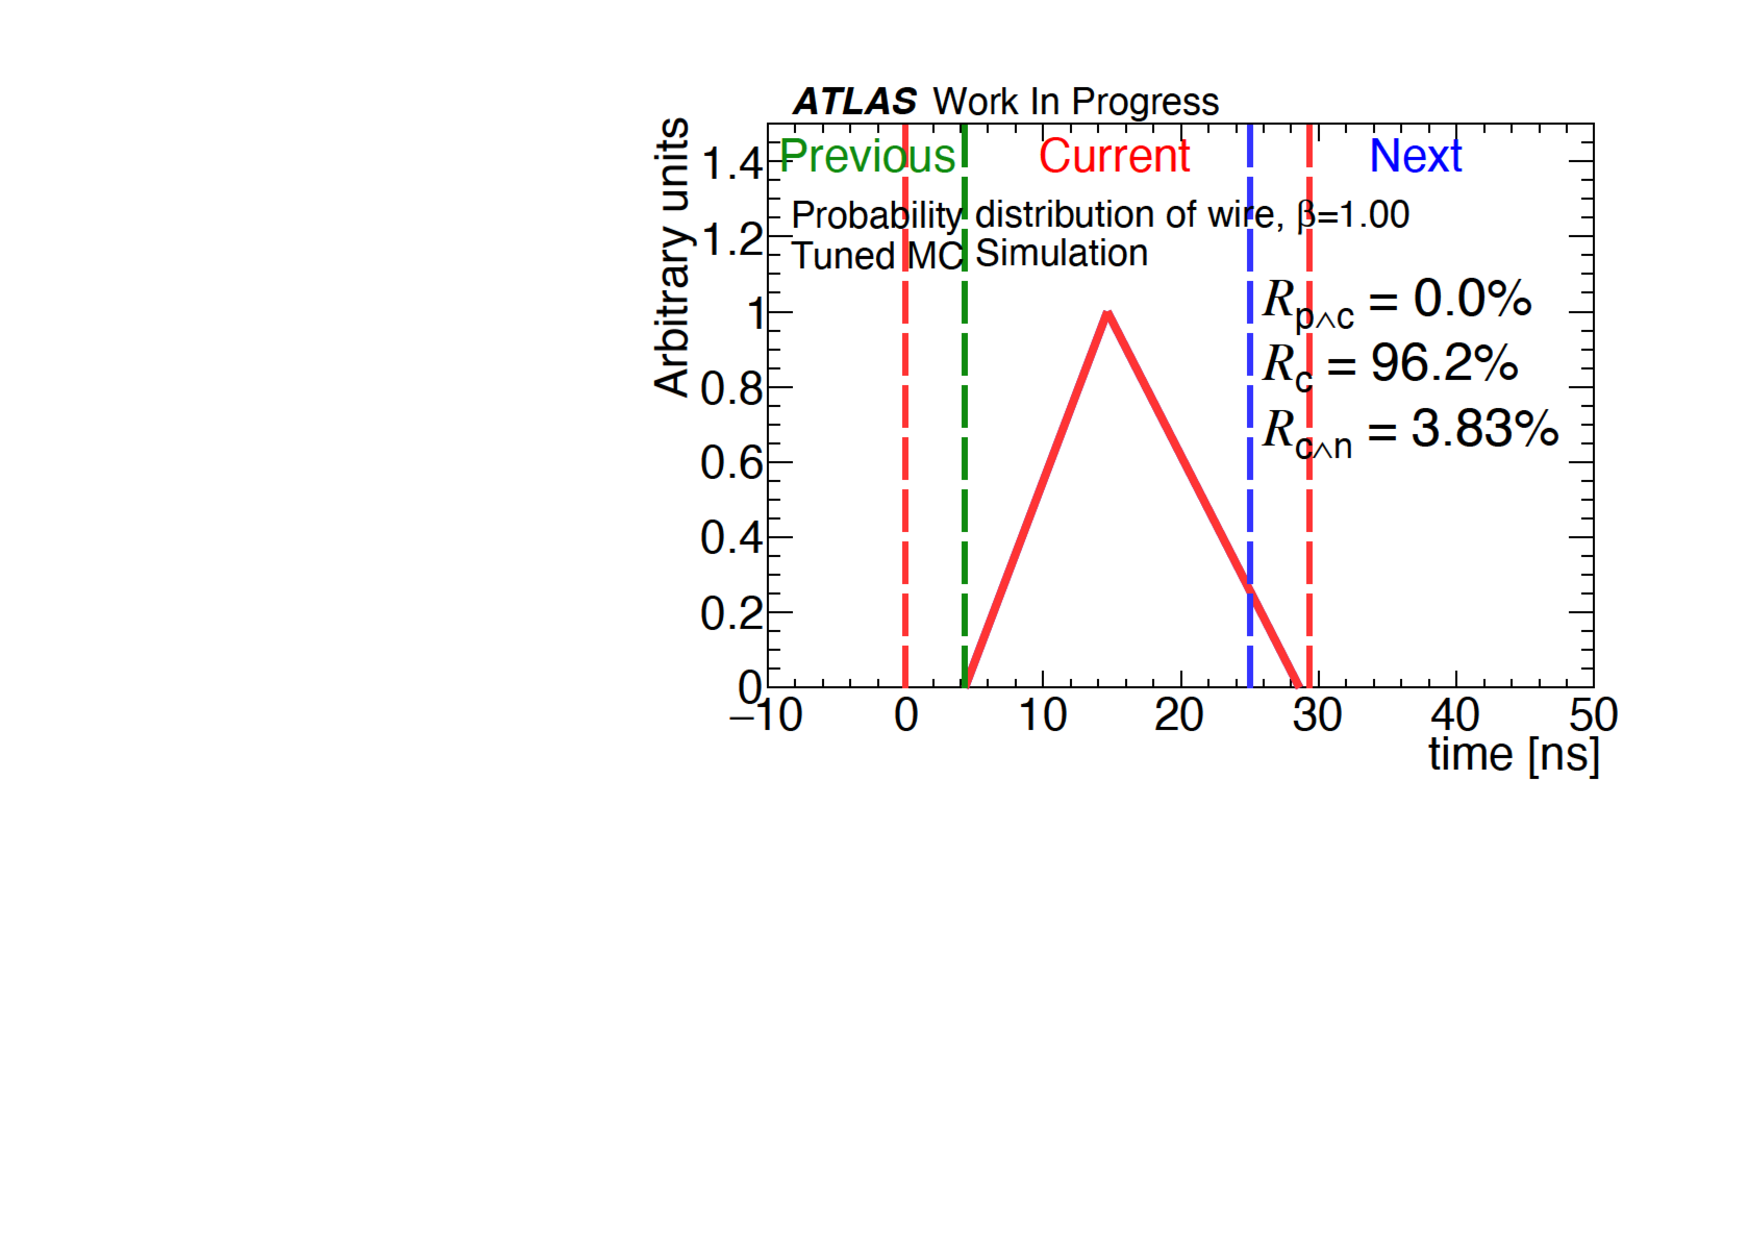
\includegraphics[width=\textwidth,page=1]{img/rec/rec_tune_w.pdf}
    \subcaption{}
    \end{minipage}
    \begin{minipage}{0.49\hsize}
    \centering   
    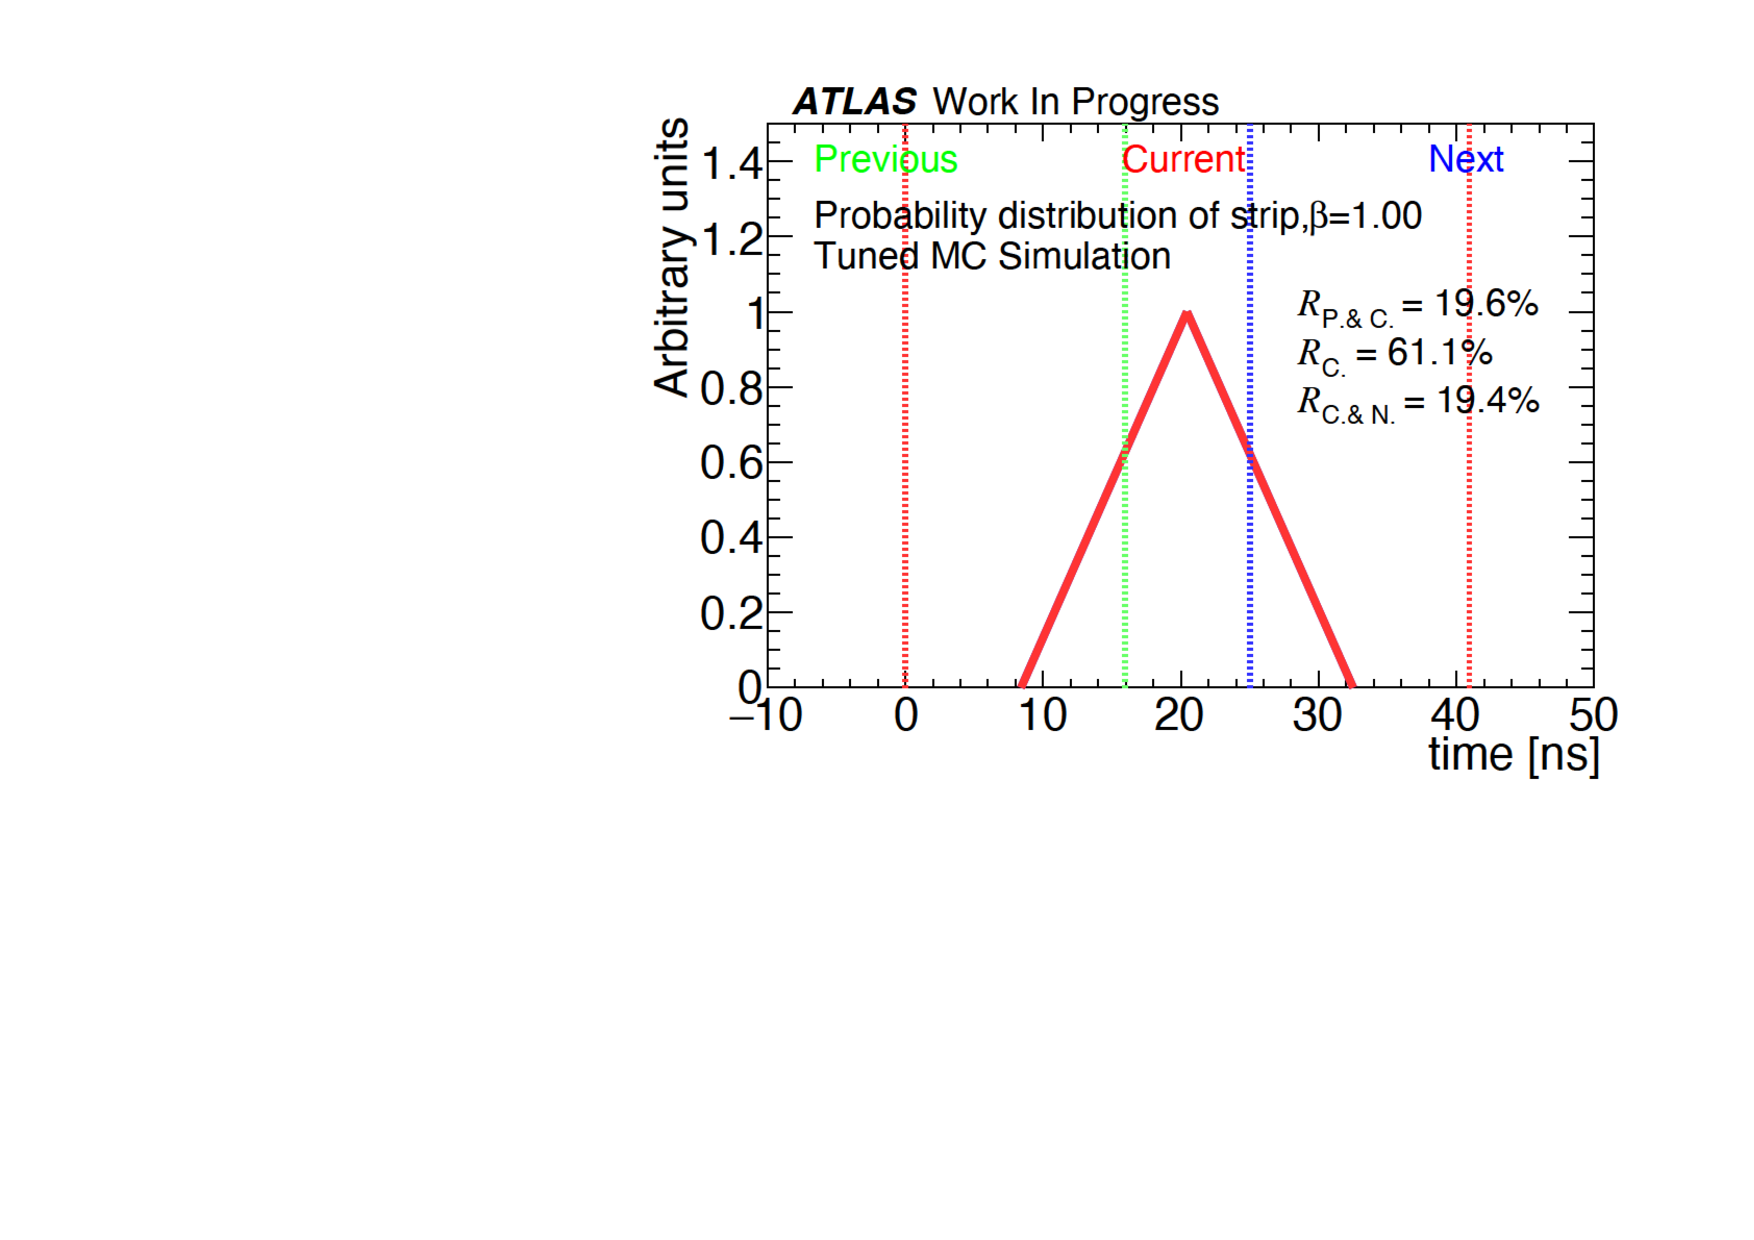
\includegraphics[width=\textwidth,page=1]{img/rec/rec_tune_s.pdf}
    \subcaption{}
    \end{minipage}
    \caption[バンチ判定から推定した較正後のシミュレーションにおけるヒットタイミングの確率分布]{バンチ判定から推定した較正後のシミュレーションにおけるヒットタイミングの確率分布。$R_{\rm{P.\&~C.}},~R_{\rm{C.}},~R_{\rm{C.\&~N.}}$~はそれぞれ前かつ基準バンチ、基準バンチ、基準かつ次のバンチの確率分布における割合を示している。(a)~M1~wire~チャンネル。(b)~M1~strip~チャンネル。}\label{fig:rectune}
\end{figure}

\subsubsection{粒子速度と確率分布}\label{sec:prob}
前節で求めた確率分布関数は~$\beta=1.0$~のミューオンの確率分布であると考えることができる。速度の遅い粒子における確率分布を考える場合は、上記のミューオンに対してどれだけ遅れているかという指標をもとに算出することができる。例えば、TGC~の任意のチェンバーに対して速度の遅い粒子が到達する場合を仮定する。このとき、速度の遅い粒子と光速の粒子の同じ場所での到達時間差が計算上、$t$~であったとする。すると任意のチェンバーに対する速度の遅い粒子の確率分布は、光速のミューオンの確率分布を~$t$~だけ遅らせたものであると考えられる。以上の仮定をもとに粒子速度と到達時間の関係から速度の遅い粒子の確率分布を見積もる。

粒子の飛来時間は~TGC~の位置と飛来する角度によって異なる。そこで\figref{fig:velo}に示すように飛来時間が短い~M1~と飛来時間が長い~M3~での角度ごとによる粒子の到達時間を考え、確率分布を見積もった。角度に関しては、エンドキャップ領域において~$\eta$~を~0.1~毎に分割して考え、各角度での粒子到達時間を計算した。\figref{fig:recbeta}、\figref{fig:recbeta1}は任意の角度方向において粒子速度の変化により確率分布がどのように変化するかを表した図である。M1~と~M3~での確率分布を算出し両者の確率のかけ合わせにより、トリガーできる割合を見積もる。
\begin{figure}[H]
    \centering   
    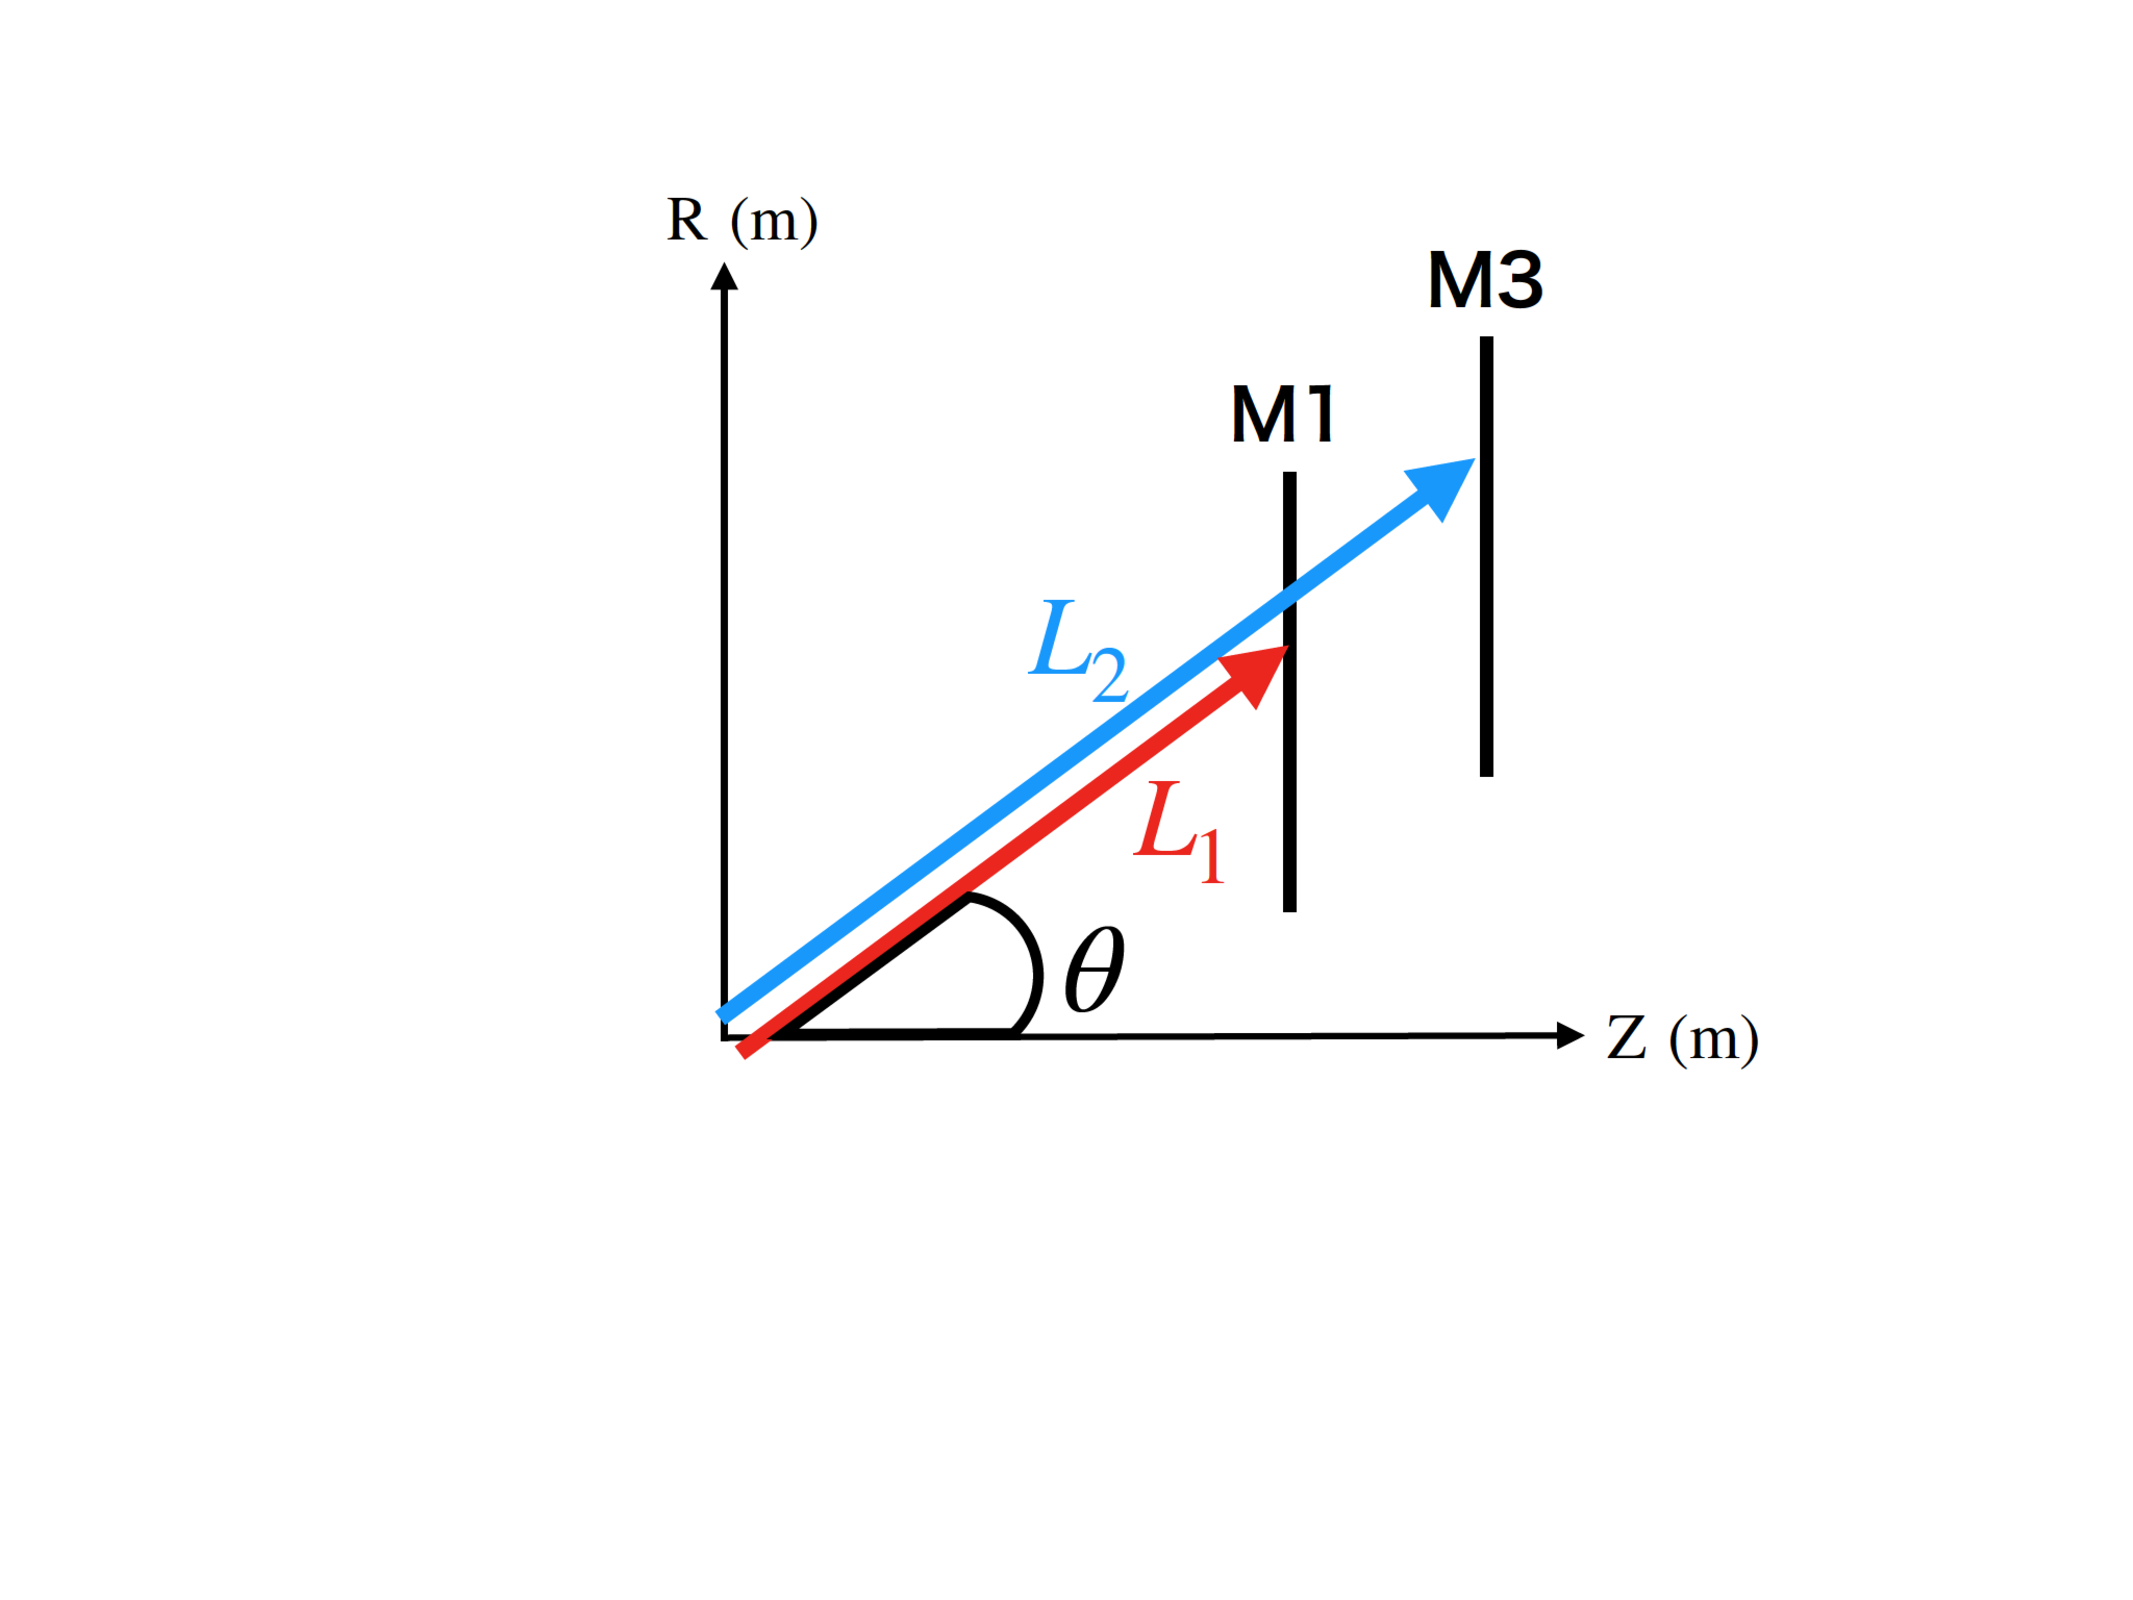
\includegraphics[width=0.7\textwidth,page=1]{img/slide/BX.pdf}
    \caption{衝突点から~TGC~検出器までの粒子到達の様子}\label{fig:velo}
\end{figure}

\begin{figure}[H]
    \begin{minipage}{0.33\hsize}
    \centering   
    \includegraphics[width=\textwidth,page=11]{img/rec/rec_e1.3_s.pdf}
    \subcaption{}
    \end{minipage}
    \begin{minipage}{0.33\hsize}
    \centering   
    \includegraphics[width=\textwidth,page=9]{img/rec/rec_e1.3_s.pdf}
    \subcaption{}
    \end{minipage}
    \begin{minipage}{0.33\hsize}
    \centering   
    \includegraphics[width=\textwidth,page=7]{img/rec/rec_e1.3_s.pdf}
    \subcaption{}
    \end{minipage}
    \caption[$|\eta|~=~1.3$~における粒子速度に依存した確率分布の変化]{$|\eta|~=~1.3$~における粒子速度に依存した確率分布の変化。赤が~M1~における確率分布、青が~M3~における確率分布を示している。(a)~$\beta~=~1.0$。(a)~$\beta~=~0.8$。(c)~$\beta~=~0.6$。}\label{fig:recbeta}
\end{figure}

\begin{figure}[H]
    \begin{minipage}{0.33\hsize}
    \centering   
    \includegraphics[width=\textwidth,page=11]{img/rec/rec_e2.2_s.pdf}
    \subcaption{}
    \end{minipage}
    \begin{minipage}{0.33\hsize}
    \centering   
    \includegraphics[width=\textwidth,page=9]{img/rec/rec_e2.2_s.pdf}
    \subcaption{}
    \end{minipage}
    \begin{minipage}{0.33\hsize}
    \centering   
    \includegraphics[width=\textwidth,page=7]{img/rec/rec_e2.2_s.pdf}
    \subcaption{}
    \end{minipage}
    \caption[$|\eta|~=~2.2$~における粒子速度に依存した確率分布の変化]{$|\eta|~=~2.2$~における粒子速度に依存した確率分布の変化。赤が~M1~における確率分布、青が~M3~における確率分布を示している。(a)~$\beta~=~1.0$。(a)~$\beta~=~0.8$。(c)~$\beta~=~0.6$。}\label{fig:recbeta1}
\end{figure}

\subsubsection{トリガー効率の算出}\label{sec:prot}
\figref{fig:recbeta}ではシミュレーションにおける速度による確率分布の変化について見積もった。$\beta=1.0$~の場合は、\figref{fig:rectune}の分布と同じである。この図では、横軸の時間軸に対して、前のバンチ、基準バンチ、次のバンチの~BCID~ゲートが設定されている。従って、確率分布の三角形がどれだけの割合でバンチ識別のタイミングにおいてどこに位置しているのかを見積もることで、トリガーできる割合を間接的に算出することができる。基準バンチに含まれる割合がシングルミューオントリガーのトリガー効率となり、次のバンチに含まれる割合が遅い荷電粒子探索用トリガーのトリガー効率となると考えられる。
\figref{fig:efftune}は、上記の確率分布より算出したトリガー効率である。wire,~strip~それぞれにトリガー効率を算出し、効率を掛け合わせることによって全体のトリガー効率を見積もる。
次節では、上記の流れで見積もることができたトリガー効率をモンテカルロシミュレーションで得られた効率と比較し、トリガー効率の見積もり手法の評価を行う。
\begin{figure}[H]
    \begin{minipage}{0.49\hsize}
    \centering   
    \includegraphics[width=\textwidth,page=2]{img/rec/eff_wire.pdf}
    \subcaption{}
    \end{minipage}
    \begin{minipage}{0.49\hsize}
    \centering   
    \includegraphics[width=\textwidth,page=2]{img/rec/eff_strip.pdf}
    \subcaption{}
    \end{minipage} \\
    \begin{minipage}{0.99\hsize}
    \centering   
    \includegraphics[width=0.5\textwidth,page=2]{img/rec/eff_both.pdf}
    \subcaption{}
    \end{minipage}
    \caption[較正後のシミュレーションにおける見積もり手法を用いたトリガー効率の算出]{較正後のシミュレーションにおける見積もり手法を用いたトリガー効率の算出。赤は~L1~シングルミューオントリガー、青は遅い荷電粒子探索用トリガーを想定して見積もられたトリガー効率。(a)~wire~の確率分布から得られたトリガー効率。(b)~strip~の確率分布から得られたトリガー効率。(c)~wire,~strip~のトリガー効率を掛け合わせ見積もった全体のトリガー効率。}\label{fig:efftune}
\end{figure}


\subsubsection{トリガー効率の見積もり手法の評価}\label{chap:caltri}
タイミング較正後のシミュレーションを利用して、粒子速度に依存したトリガー効率の見積もり手法の評価を行った。\figref{fig:comp}は、見積もり手法を利用して算出したトリガー効率とモンテカルロシミュレーションによって得られたデータから求めたトリガー効率の比較である。見積もり手法から得られたトリガー効率に関しては、シングルミューオントリガーで最大効率が~$80~\%$、遅い荷電粒子用トリガーで最大効率が~$30~\%$~となるように較正を行っている。$\beta$~方向におけるトリガー可能な領域に良い一致がみられていることがわかる。この手法を用いて~Run~2~の実験データで期待されるトリガー効率を算出していく。

\begin{figure}[H]
    \centering   
    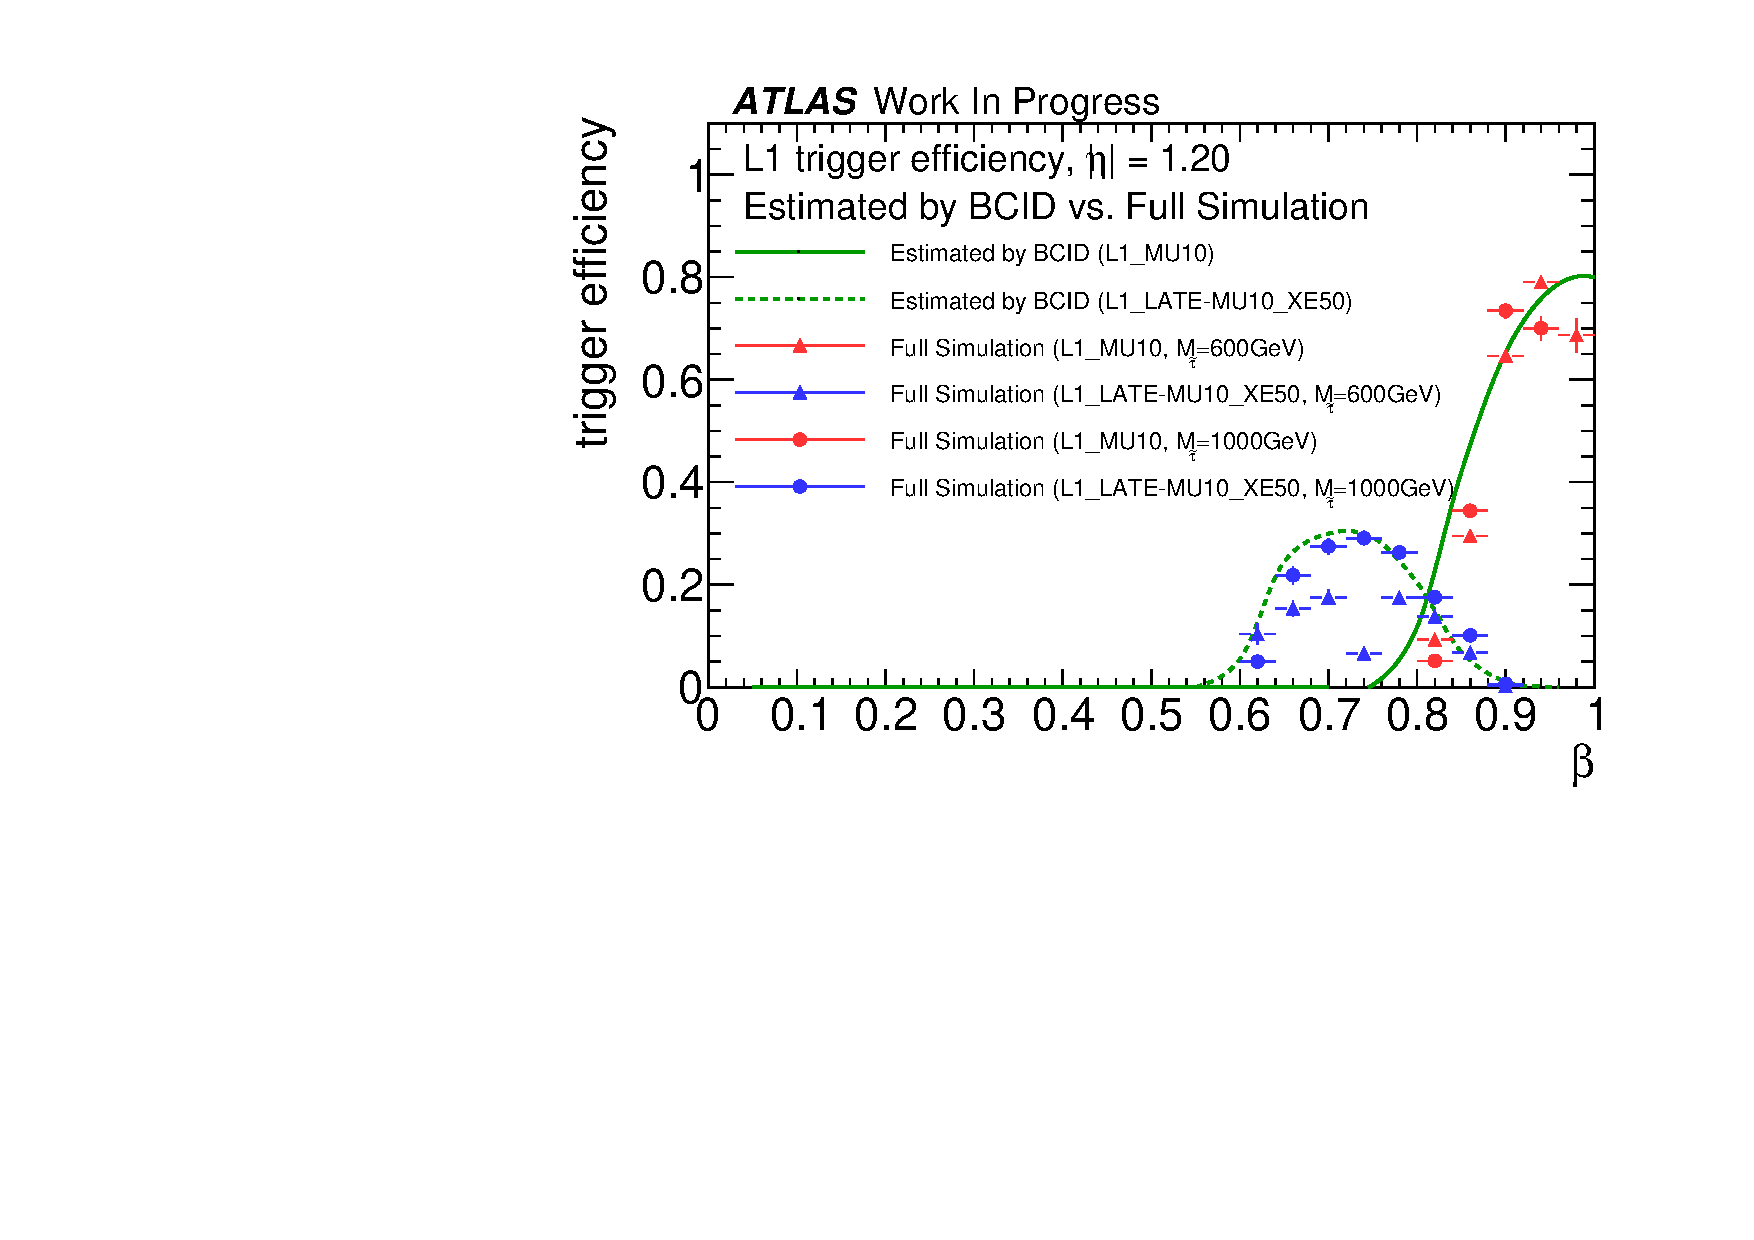
\includegraphics[width=0.8\textwidth,page=1]{img/rec/vs.pdf}
    \caption[トリガー効率見積もり手法とフルモンテカルロシミュレーションのトリガー効率の比較]{トリガー効率見積もり手法とフルモンテカルロシミュレーションのトリガー効率の比較。緑の実線は見積もり手法から算出したシングルミューオントリガー、破線は遅い荷電粒子探索用トリガー、赤はフルモンテカルロシミュレーションにおけるシングルミューオントリガー、青は遅い荷電粒子探索用トリガーのトリガー効率を示す。▲はスタウサンプルの質量~600~GeV、●はスタウサンプルの質量~1000~GeV。}\label{fig:comp}
\end{figure}

\subsection{見積もり手法を利用したRun~2~データとシミュレーションの比較}
\secref{sec:est}で説明したバンチ判定を利用したトリガー効率の見積もり手法を用いて、実際に~Run~2~のデータにおけるトリガー効率を算出する。シミュレーションを用いて得られたトリガー効率との差を比較することで、シミュレーションの評価を行う。
\subsubsection{確率分布関数の定義}
\secref{sec:pro}で説明した確率分布関数の定義方法を利用して、Run~2~データおよびタイミング較正前後のシミュレーションにおける確率分布関数を定義する。定義のために必要なバンチ判定の分布には、\subsecref{chap:caltri}において記載した結果を利用している。確率分布関数の算出結果を\figref{fig:recall}並びに\figref{fig:recall1}に示す。実験データ、シミュレーションそれぞれに求めた確率分布関数をもとに、\secref{sec:prob}で述べた粒子速度に依存した確率分布の見積もりの計算を行い、トリガー効率を\secref{sec:prot}の要領で算出する。

\begin{figure}[H]
    \begin{minipage}{0.33\hsize}
    \centering   
    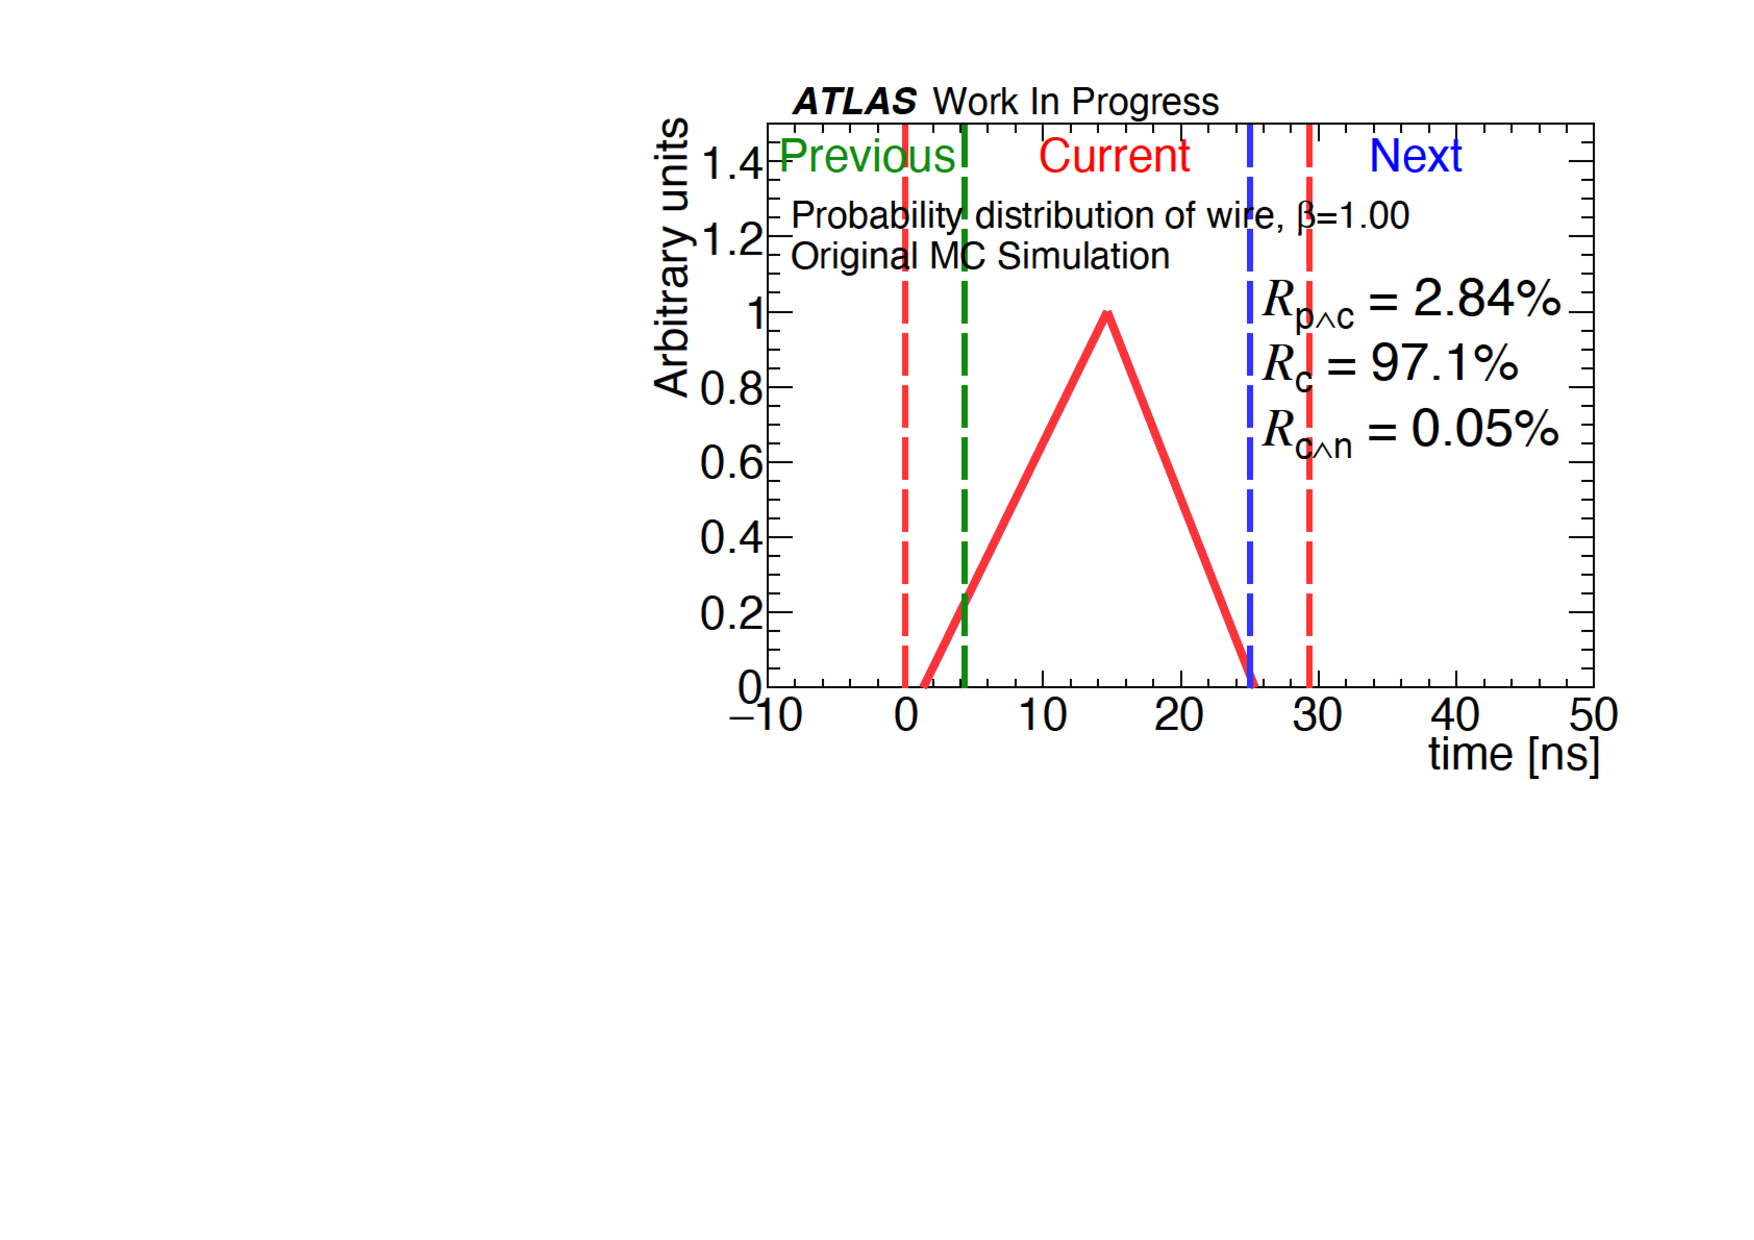
\includegraphics[width=\textwidth,page=1]{img/rec/rec_ori_w.pdf}
    \subcaption{}
    \end{minipage}
    \begin{minipage}{0.33\hsize}
    \centering   
    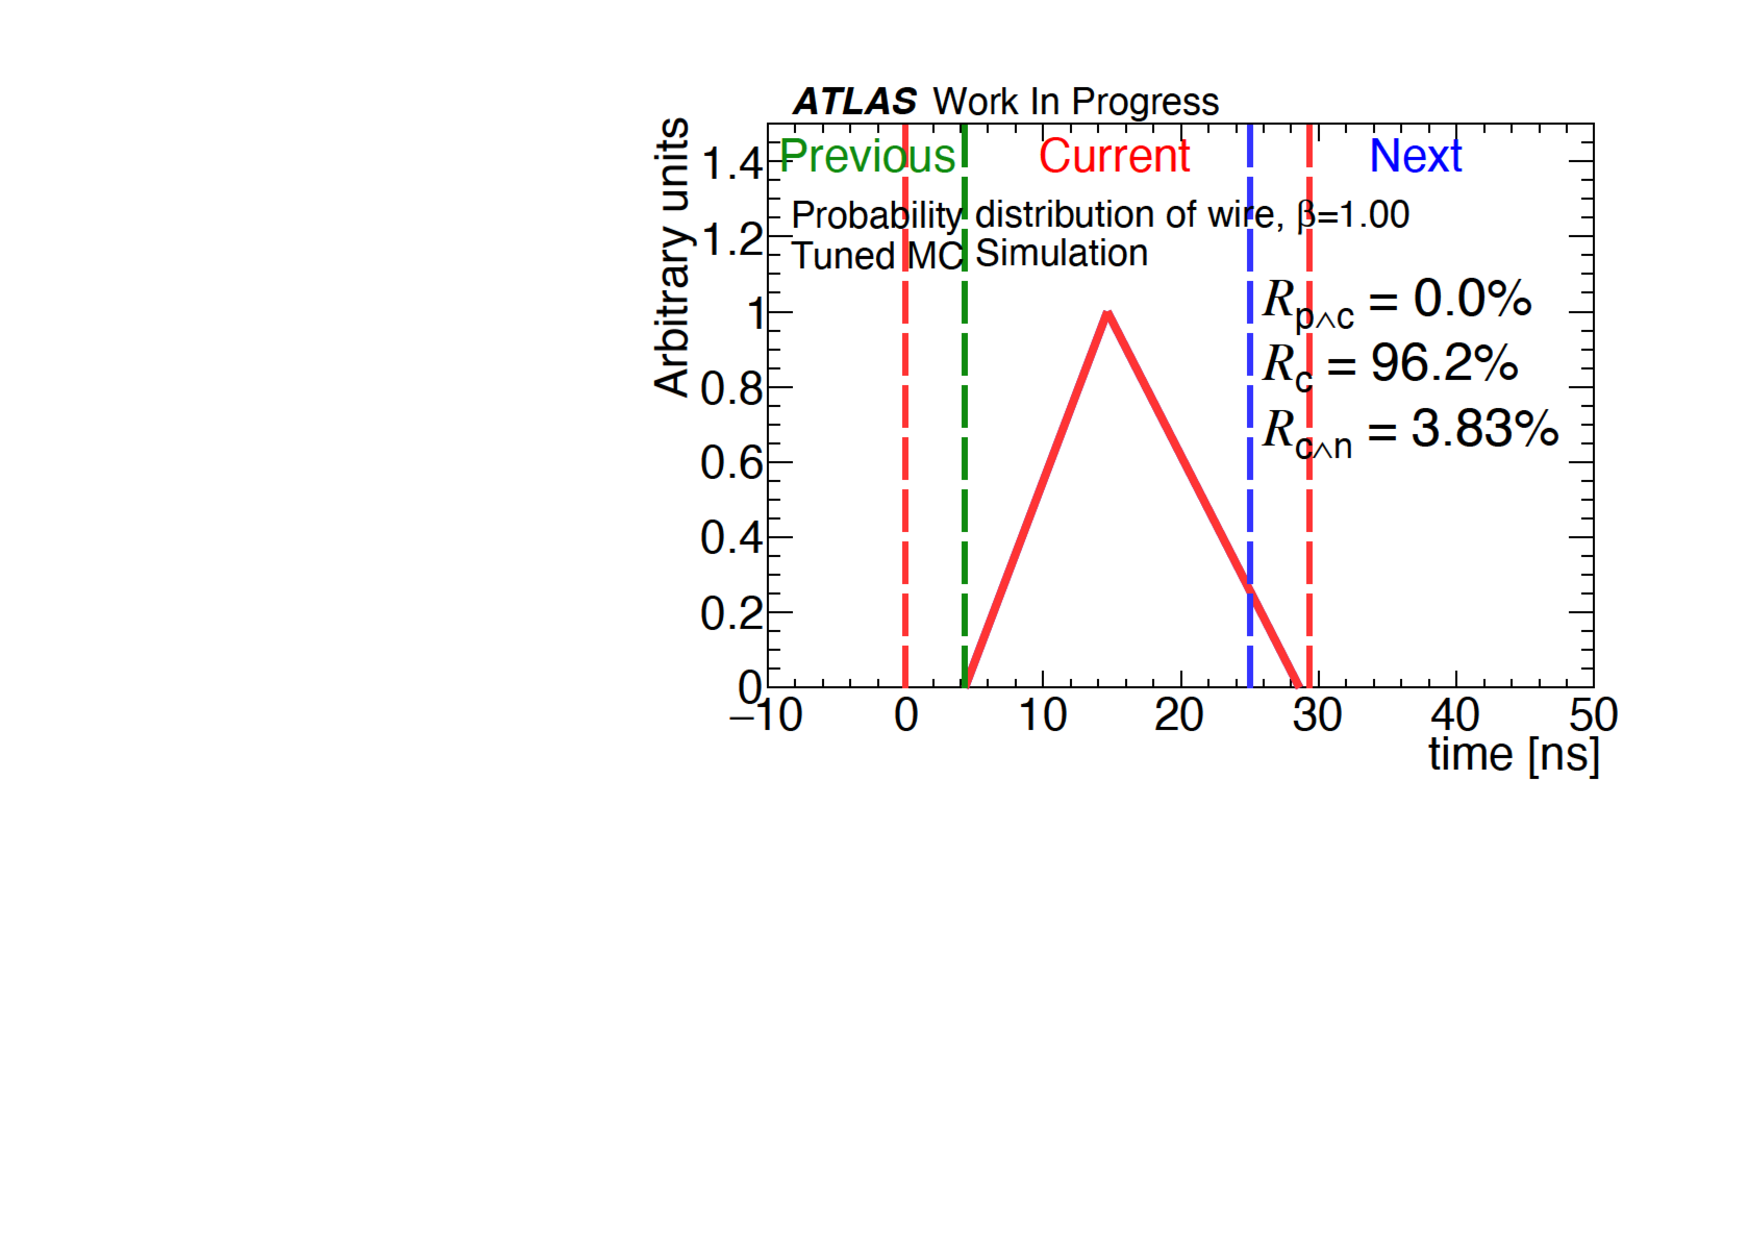
\includegraphics[width=\textwidth,page=1]{img/rec/rec_tune_w.pdf}
    \subcaption{}
    \end{minipage}
    \begin{minipage}{0.33\hsize}
    \centering   
    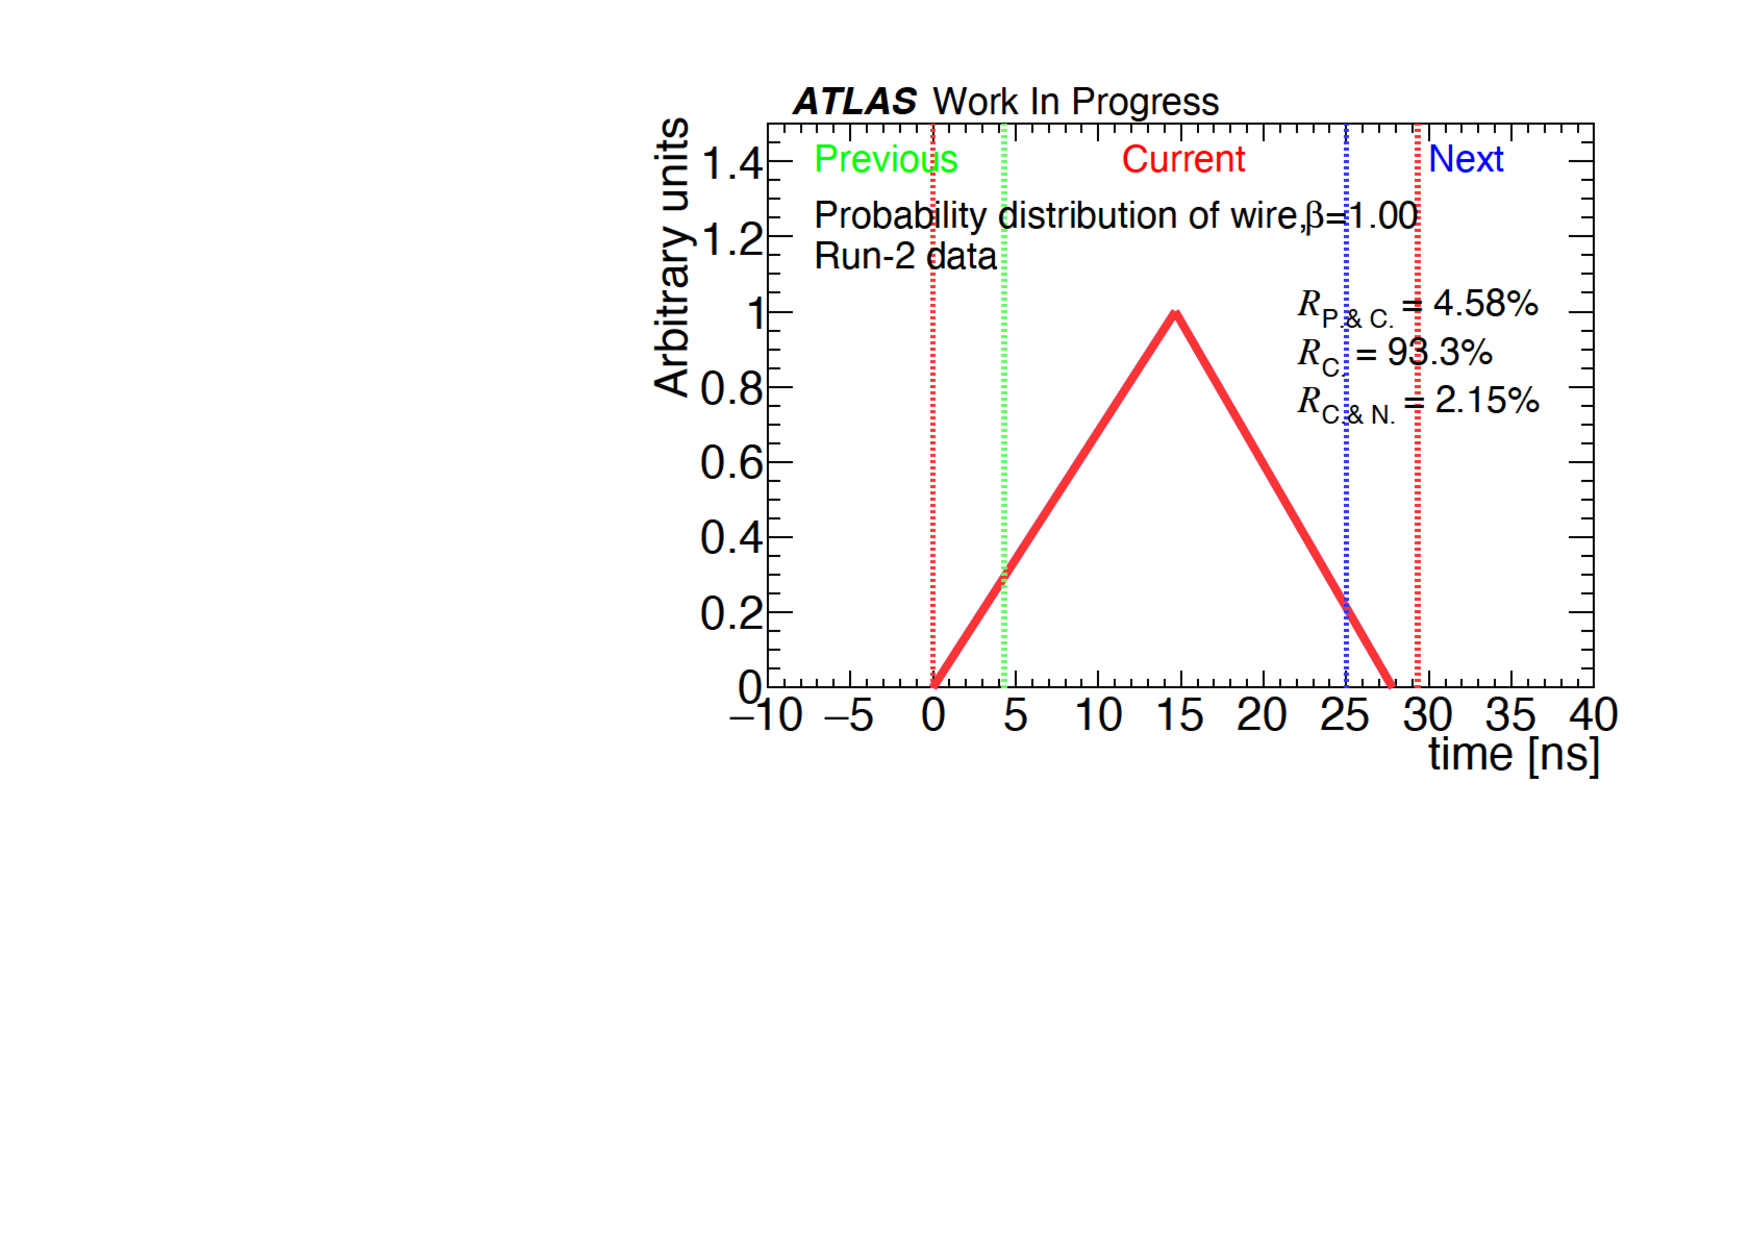
\includegraphics[width=\textwidth,page=1]{img/rec/rec_data_w.pdf}
    \subcaption{}
    \end{minipage}
    \caption[実験データおよびシミュレーションにおけるバンチ判定から推定した~wire~のヒットタイミングの確率分布]{実験データおよびシミュレーションにおけるバンチ判定から推定した~wire~のヒットタイミングの確率分布。$R_{\rm{P.\&~C.}},~R_{\rm{C.}},~R_{\rm{C.\&~N.}}$~はそれぞれ前かつ基準バンチ、基準バンチ、基準かつ次のバンチの確率分布における割合を示している。(a)~較正前のシミュレーション。(b)較正後のシミュレーション。(c)~Run~2~実験データ。}\label{fig:recall}
\end{figure}

\begin{figure}[H]
    \begin{minipage}{0.33\hsize}
    \centering   
    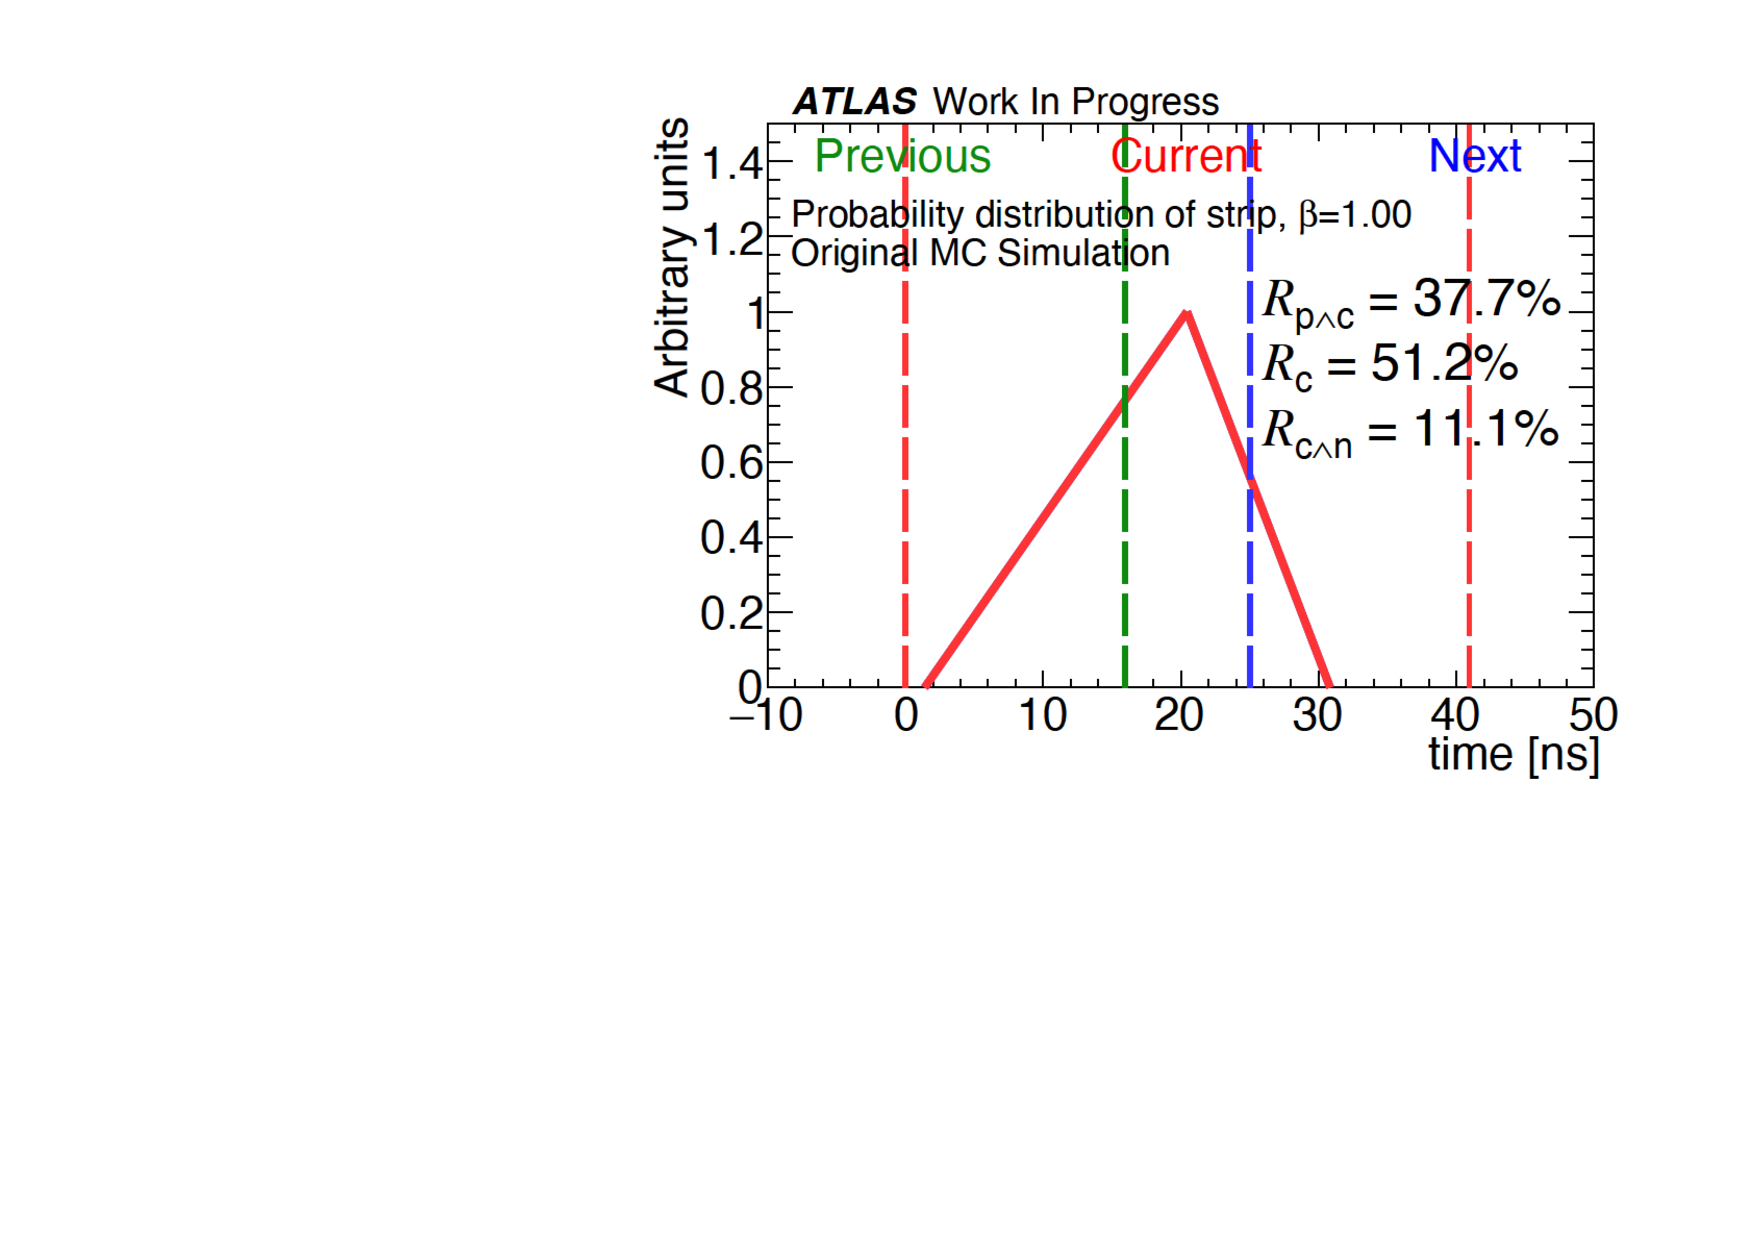
\includegraphics[width=\textwidth,page=1]{img/rec/rec_ori_s.pdf}
    \subcaption{}
    \end{minipage}
    \begin{minipage}{0.33\hsize}
    \centering   
    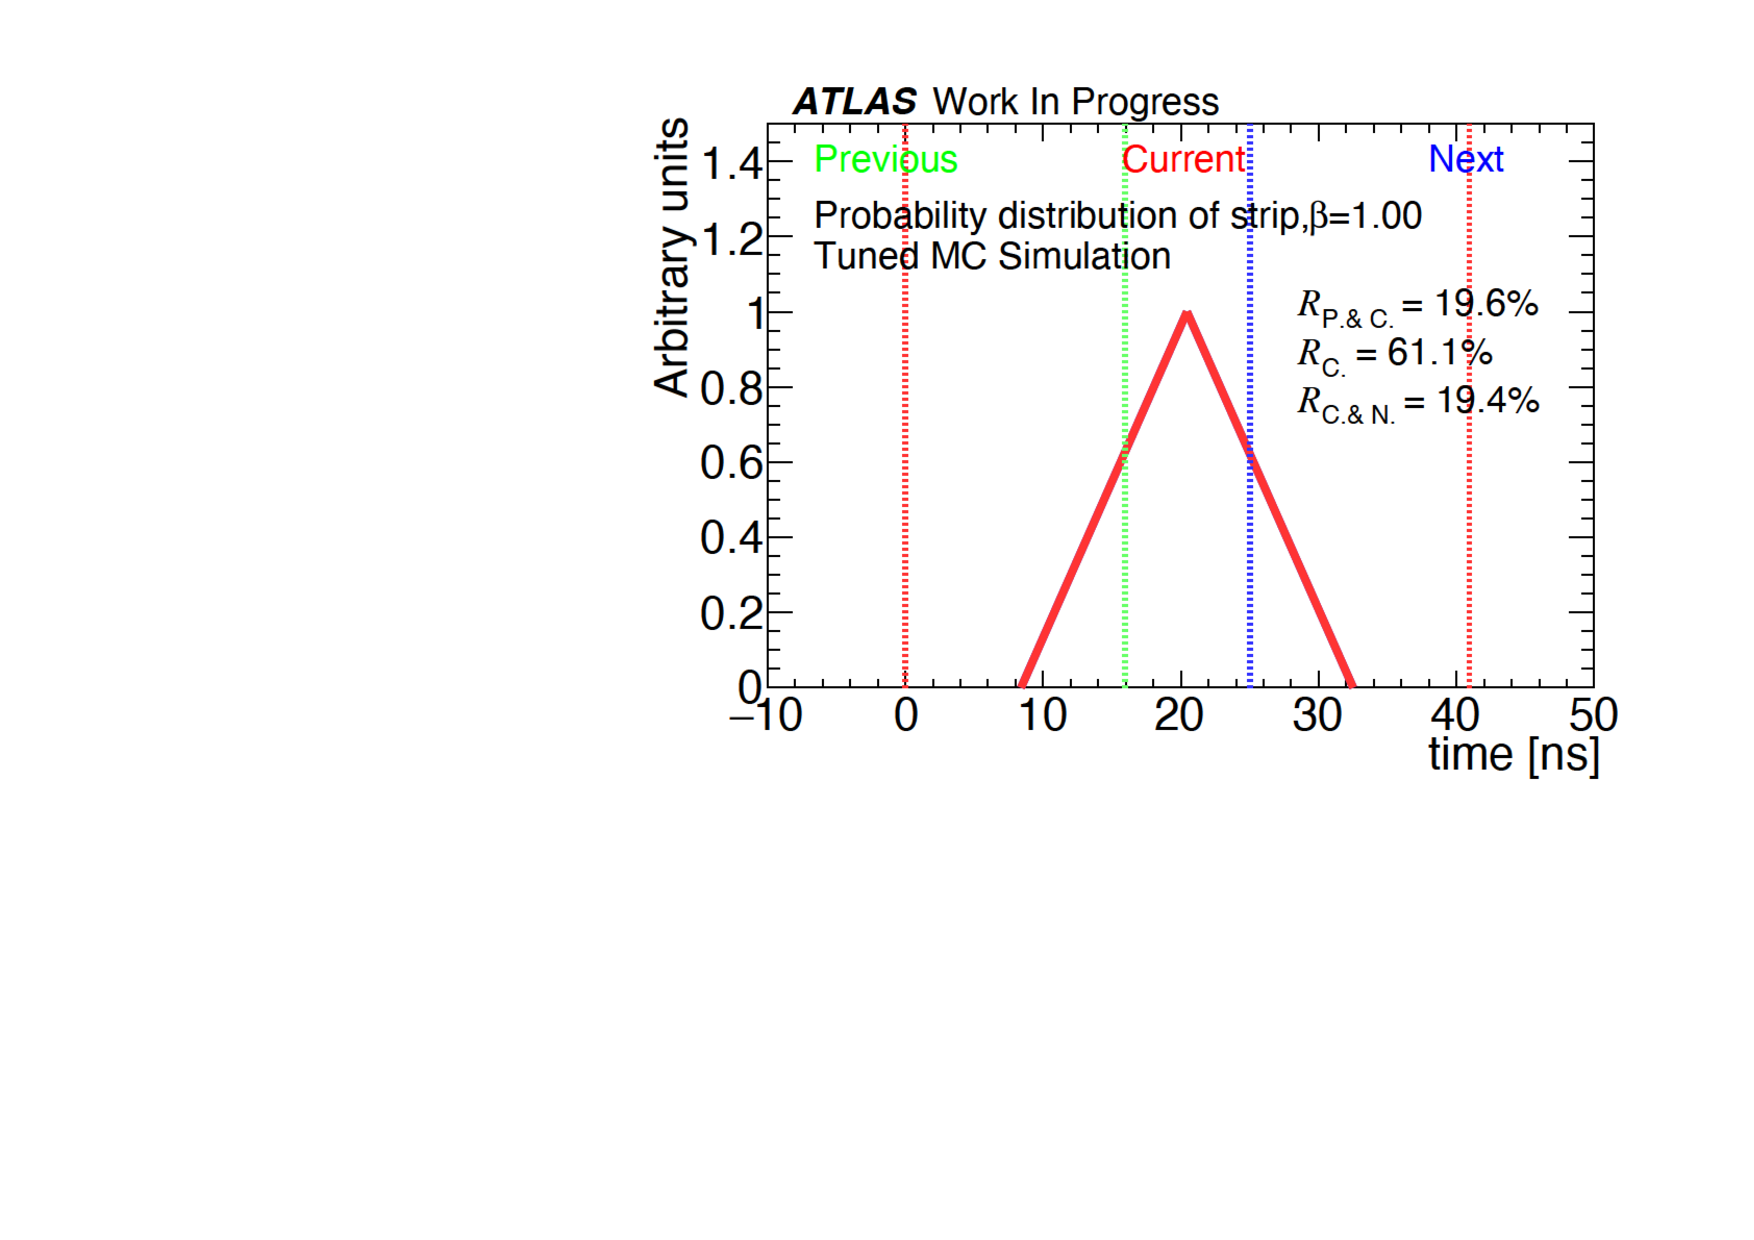
\includegraphics[width=\textwidth,page=1]{img/rec/rec_tune_s.pdf}
    \subcaption{}
    \end{minipage}
    \begin{minipage}{0.33\hsize}
    \centering   
    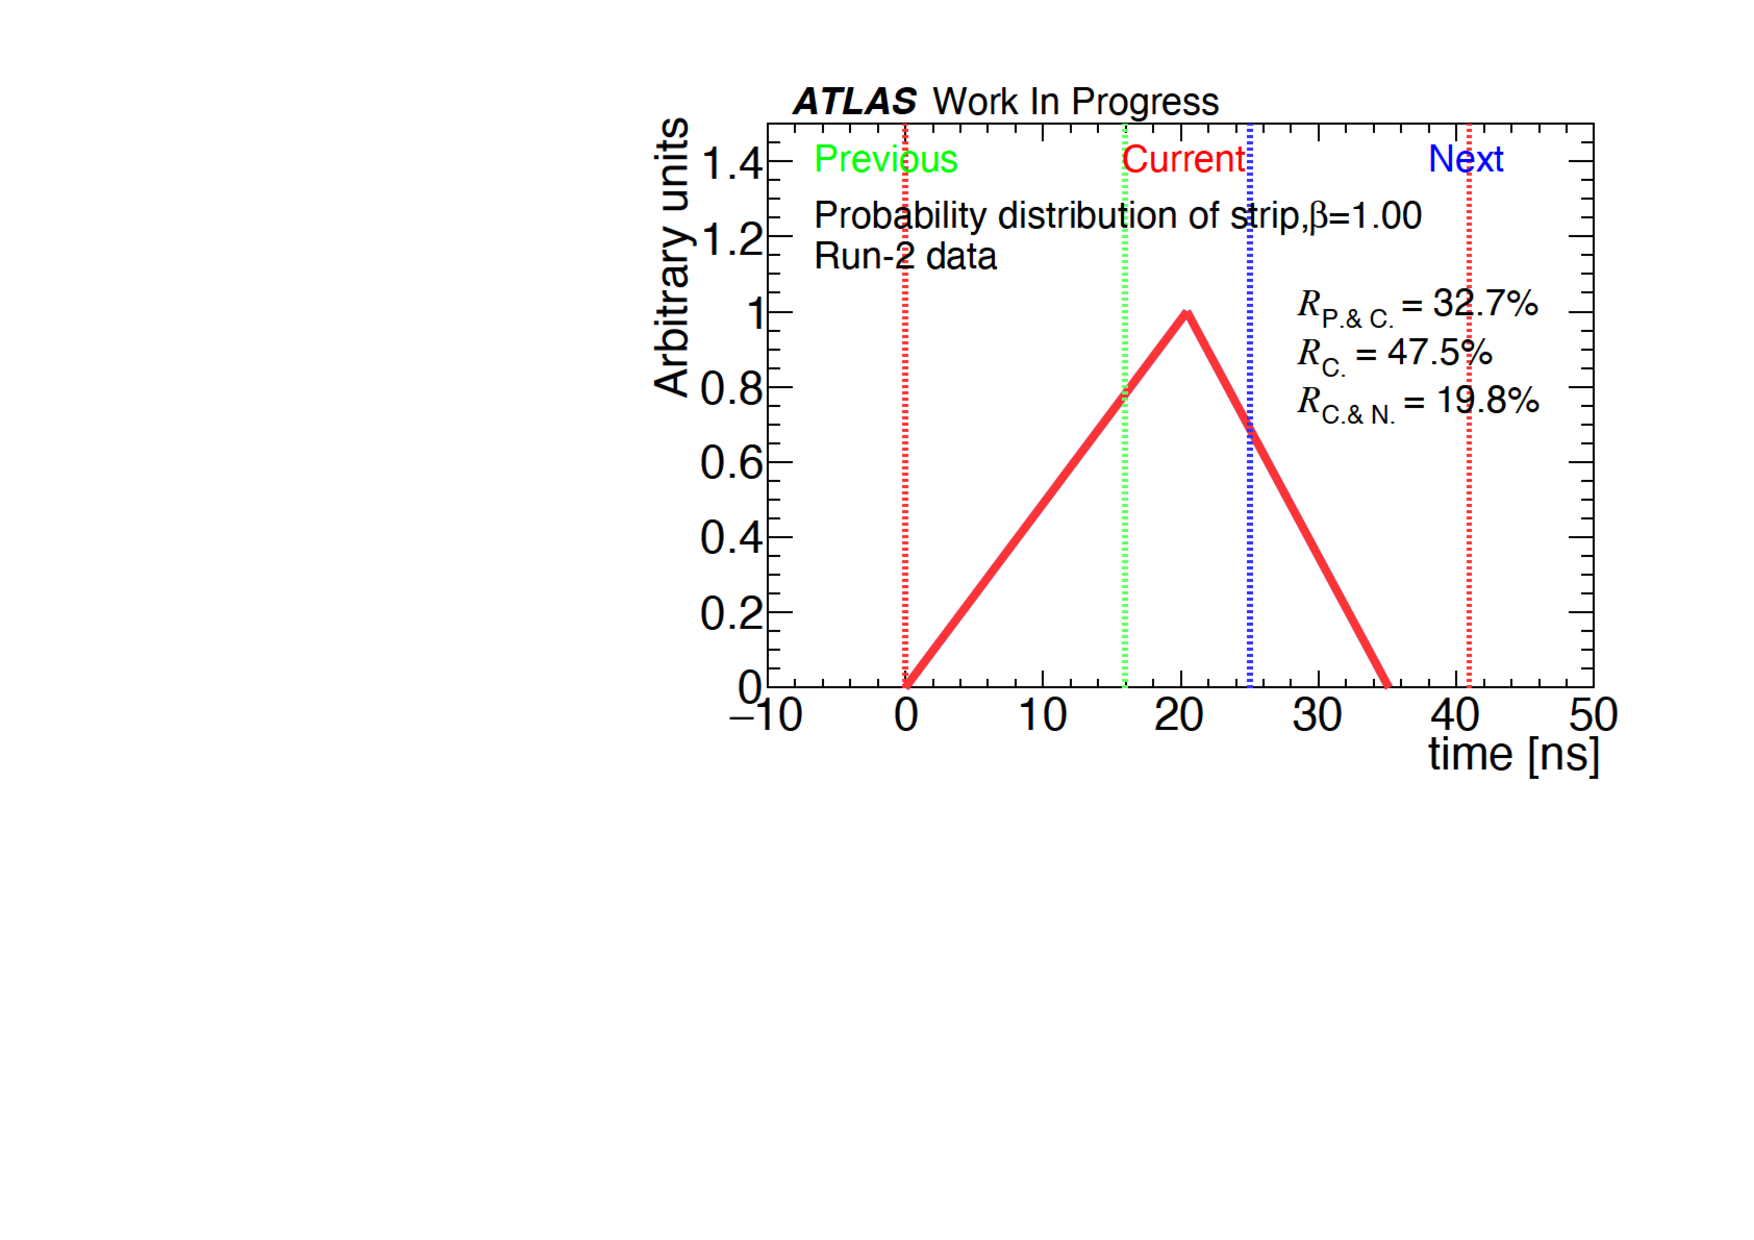
\includegraphics[width=\textwidth,page=1]{img/rec/rec_data_s.pdf}
    \subcaption{}
    \end{minipage} 
    \caption[実験データおよびシミュレーションにおけるバンチ判定から推定した~strip~のヒットタイミングの確率分布]{実験データおよびシミュレーションにおけるバンチ判定から推定した~strip~のヒットタイミングの確率分布。$R_{\rm{P.\&~C.}},~R_{\rm{C.}},~R_{\rm{C.\&~N.}}$~はそれぞれ前かつ基準バンチ、基準バンチ、基準かつ次のバンチの確率分布における割合を示している。(a)~較正前のシミュレーション。(b)較正後のシミュレーション。(c)~Run~2~実験データ。}\label{fig:recall1}
\end{figure}

\subsubsection{見積もり手法を用いたトリガー効率の比較}
Run~2~における実験データおよびタイミング較正前後のシミュレーションそれぞれにおける見積もり手法をもとに算出したトリガー効率の比較を\figref{fig:rectri}に示した。トリガー効率の見積もり手法を用いることで、データとシミュレーションの比較を行うことができ、Run~2~における実験データの評価を行うことが可能となる。BCID~分布を利用することで、新しい発想での粒子速度に依存したトリガー効率の評価方法を確立することができた。

物理解析を行う場合、系統的な不確かさに起因する一つの要因として、実験データとモンテカルロシミュレーションの差が挙げられる。本研究では Run~2~の実験データにおけるトリガー効率を見積もるにあたり、新たなトリガー効率の見積もり手法を用いた。このとき系統誤差として、実験データとシミュレーションにおける見積もったトリガー効率の差が影響する。また、シミュレーションにおける見積もり手法からのトリガー効率と完全なモンテカルロシミュレーションから算出したトリガー効率の差に関しても系統誤差に起因する。\figref{fig:rectritune}には、見積もり手法から算出した Run~2~の実験データおよび較正後のシミュレーションのトリガー効率と完全なモンテカルロシミュレーションから算出したトリガー効率の比較を示した。

本研究では~TGC~検出器のタイミング較正により、より詳細な実験の再現を行うことに成功した。また、実験データの新しいトリガー効率評価手法を確立した。以上により~Run~3~においては、重い長寿命荷電粒子探索において、より不確かさの少ない物理解析が行えることが期待できる。
\begin{figure}[H]
    \centering   
    \includegraphics[width=\textwidth,page=4]{img/rec/est_eff.pdf}
    \caption[トリガー効率の見積もり手法から算出したシミュレーションおよび実験データにおけるトリガー効率の比較]{トリガー効率の見積もり手法から算出したシミュレーションおよび実験データにおけるトリガー効率の比較。$|\eta|~=~1.2$。実線はシングルミューオントリガー、破線は遅い荷電粒子探索用トリガーの見積もり手法から算出されたトリガー効率を示す。緑は較正後のシミュレーション、青は較正前のシミュレーション、橙は~Run~2~実験データを表す。}\label{fig:rectri}
\end{figure}

\begin{figure}[H]
    \centering   
    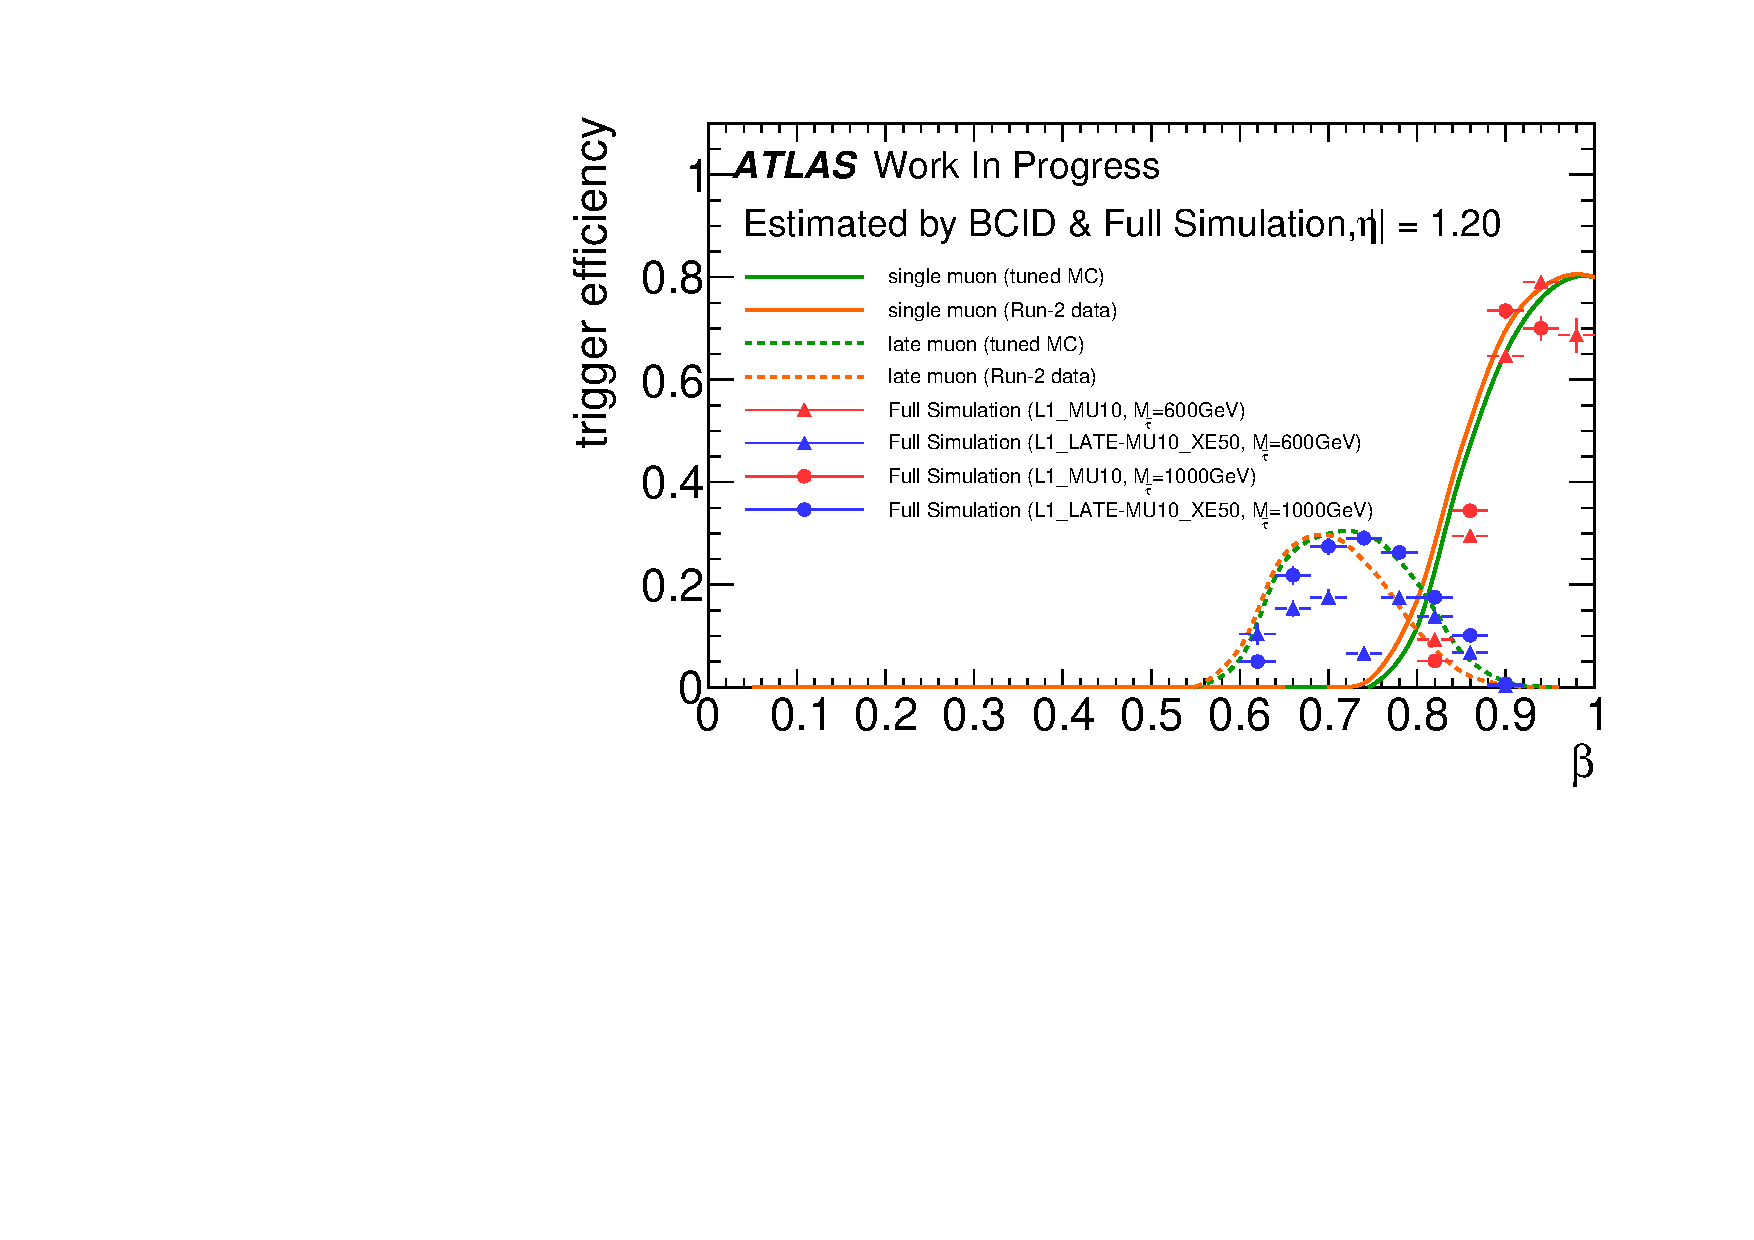
\includegraphics[width=\textwidth,page=1]{img/rec/tunetune.pdf}
    \caption[トリガー効率の見積もり手法から算出したシミュレーションおよび実験データにおけるトリガー効率とフルモンテカルロシミュレーションにおけるトリガー効率の比較]{トリガー効率の見積もり手法から算出したシミュレーションおよび実験データにおけるトリガー効率とフルモンテカルロシミュレーションにおけるトリガー効率の比較。$|\eta~=~1.2|$。実線はシングルミューオントリガー、破線は遅い荷電粒子探索用トリガーの見積もり手法から算出されたトリガー効率を示す。緑は較正後のシミュレーション、橙は~Run~2~実験データを表す。点はフルモンテカルロシミュレーションによるトリガー効率を示し、赤はシングルミューオントリガー、青は遅い荷電粒子探索用トリガーのトリガー効率を示す。▲はスタウサンプルの質量~600~GeV、●はスタウサンプルの質量~1000~GeV。}\label{fig:rectritune}
\end{figure}
